\documentclass[12pt,a4paper]{report}

\usepackage[utf8]{inputenc}
\usepackage[T5]{fontenc}
\usepackage[vietnamese]{babel}
\usepackage{mathptmx}
\usepackage[top=2.2cm,bottom=2.2cm,left=2.5cm,right=2.5cm]{geometry}
\usepackage{graphicx}
\usepackage{float}
\usepackage{booktabs}
\usepackage{longtable}
\usepackage{array}
\usepackage{xcolor}
\usepackage{tikz}
\usepackage{fancyhdr}
\usepackage{titlesec}
\usepackage{enumitem}
\usepackage{amsmath,amssymb}
\usepackage{caption}
\usepackage{pifont}
\usepackage[unicode,colorlinks=true,linkcolor=hcmutblue,urlcolor=hcmutblue,citecolor=hcmutblue]{hyperref}

\definecolor{hcmutblue}{HTML}{003366}
\definecolor{hcmutsub}{HTML}{005599}
\definecolor{textdark}{HTML}{222222}

\renewcommand{\contentsname}{MỤC LỤC}
\setcounter{tocdepth}{2}
\setcounter{secnumdepth}{3}

% Chapter, Section, Subsection formatting
\titleformat{\chapter}[hang]{\Large\bfseries\color{hcmutblue}}{CHƯƠNG \thechapter: }{0pt}{}
\titlespacing*{\chapter}{0pt}{0pt}{14pt}
\titleformat{\section}{\large\bfseries\color{hcmutsub}}{\thesection.}{0.5em}{}
\titlespacing*{\section}{0pt}{12pt}{5pt}
\titleformat{\subsection}{\normalsize\bfseries\color{textdark}}{\thesubsection.}{0.5em}{}
\titlespacing*{\subsection}{0pt}{8pt}{4pt}

% Paragraph & Caption defaults
\setlength{\parskip}{4pt}
\setlength{\parindent}{0pt}
\renewcommand{\baselinestretch}{1.22}
\captionsetup{font={small,it},labelfont={bf},justification=centering}

% Header & Footer for main pages
\pagestyle{fancy}
\fancyhf{}
\fancyhead[R]{\small\textit{\textcolor{gray}{EE3003 -- Lớp L01 -- Nhóm 7 -- HK 261 \textbar{} Báo cáo Đồ án Hệ thống Nhúng}}}
\fancyfoot[C]{\small\textcolor{gray}{Trang \thepage}}
\renewcommand{\headrulewidth}{0.4pt}
\renewcommand{\footrulewidth}{0pt}

\begin{document}

% ============================================================
% TRANG BÌA (COVER PAGE)
% ============================================================
\begin{titlepage}
\begin{tikzpicture}[remember picture,overlay]
  \draw[line width=1.4pt]
    ([xshift=1.4cm,yshift=-1.4cm]current page.north west)
    rectangle
    ([xshift=-1.4cm,yshift=1.4cm]current page.south east);
\end{tikzpicture}

\centering
\vspace*{0.4cm}
{\fontsize{13}{16}\selectfont\textbf{ĐẠI HỌC QUỐC GIA THÀNH PHỐ HỒ CHÍ MINH}}\\[4pt]
{\fontsize{13}{16}\selectfont\textbf{TRƯỜNG ĐẠI HỌC BÁCH KHOA}}\\[4pt]
{\fontsize{14}{16}\selectfont $\cdot\cdot\cdot$\ding{72}$\cdot\cdot\cdot$}\\[1.2cm]


\includegraphics[width=4.2cm]{images/img01_bk_logo.png}\\[1.3cm]

{\fontsize{17}{21}\selectfont\textbf{BÀI TẬP LỚN}}\\[8pt]
{\fontsize{14.5}{18}\selectfont\textbf{MÔN THIẾT KẾ HỆ THỐNG NHÚNG (EE3003)}}\\[8pt]
{\fontsize{13}{16}\selectfont\textbf{LỚP L01 --- NHÓM 7 --- HK 261}}\\[14pt]
{\fontsize{12.5}{16}\selectfont\textbf{Giảng viên hướng dẫn: Nguyễn Trung Hiếu}}\\[1.1cm]

\begin{flushleft}
\hspace*{0.7cm}{\fontsize{12}{15}\selectfont Danh sách thành viên:}
\end{flushleft}
\vspace{4pt}

\renewcommand{\arraystretch}{1.45}
\begin{tabular}{|>{\centering\arraybackslash}p{1.6cm}|p{7.8cm}|>{\centering\arraybackslash}p{3.6cm}|}
\hline
\textbf{STT} & \multicolumn{1}{c|}{\textbf{Họ và tên}} & \textbf{MSSV} \\
\hline
1 & Lê Quang Dũng & 2410591 \\
\hline
2 & Trần Công Cường & 2410443 \\
\hline
3 & Phạm Ngọc Huy & 2411260 \\
\hline
\end{tabular}

\vfill
{\fontsize{12.5}{16}\selectfont\textit{Thành phố Hồ Chí Minh 2026}}
\vspace*{0.4cm}
\end{titlepage}

% ============================================================
% MỤC LỤC (TABLE OF CONTENTS)
% ============================================================
\pagenumbering{arabic}
\setcounter{page}{1}
\tableofcontents
\clearpage

\chapter{ĐẶC TẢ YÊU CẦU (REQUIREMENT FORMS)}

\section{Name}

Hệ thống tích trữ năng lượng mặt trời tích hợp bám sáng tự động (Energy Storage with Solar Tracker System).

\section{Purpose}

Tối đa hóa hiệu suất thu thập năng lượng mặt trời thông qua cơ chế tự động bám sáng, đồng thời quản lý an toàn quá trình tích trữ điện năng nhằm cung cấp nguồn điện sạc ổn định cho các khối pin và thiết bị ngoài lưới.

\section{Inputs and Outputs}

\textbf{Inputs:}
\begin{itemize}[leftmargin=1.5em,itemsep=3pt]
  \item Tín hiệu tương tự từ 4 cảm biến quang trở (LDR) qua bộ ADC 12-bit.
  \item Nguồn năng lượng 18V DC từ tấm pin mặt trời.
  \item Tín hiệu điện áp phản hồi từ khối pin lưu trữ 18650.
\end{itemize}

\textbf{Outputs:}
\begin{itemize}[leftmargin=1.5em,itemsep=3pt]
  \item Xung PWM định tuyến độc lập (qua Timer) điều khiển 2 động cơ Servo 20kg.
  \item Dòng nạp DC an toàn đã qua mạch hạ áp LM2596 cấp vào 4 pin 18650.
  \item Dữ liệu \% pin hiển thị trên màn hình OLED qua giao thức I2C.
\end{itemize}

\section{Use Cases}
\begin{itemize}[leftmargin=1.5em,itemsep=3pt]
  \item \textbf{Tự động bám sáng: }Định kỳ mỗi giây, hệ thống đọc giá trị từ 4 LDR. Nếu sai số ánh sáng vượt vùng dung sai, vi điều khiển xuất lệnh PWM xoay trục Pan và Tilt để mảng pin vuông góc với hướng nắng.
  \item \textbf{Giám sát trạng thái Pin: }Khi ánh sáng xuống thấp (mưa bão, ban đêm), hệ thống tự động ngắt nguồn Servo và đưa vi điều khiển vào chế độ ngủ để tiết kiệm pin. Hệ thống định kỳ thức dậy, đo lường điện áp pin 18650, ánh xạ ra \% và hiển thị lên màn hình.
\end{itemize}

\section{Functions}
\begin{itemize}[leftmargin=1.5em,itemsep=3pt]
  \item \textbf{Điều hướng \& Cân bằng cơ học: }Tính toán quang sai và điều khiển không gian 2 trục (Pan/Tilt) bằng cụm 2 động cơ Servo tải nặng.
  \item \textbf{Quản lý lưu trữ \& Chia tải dòng cao: }Sử dụng mạch LM2596 hạ áp từ 18V xuống 5V nạp dòng vào TP4056 để sạc cho pin 18650 và cấp ngõ ra 5V ổn định cho hệ thống.
  \item \textbf{Chế độ tiết kiệm điện: }Quản trị dòng rò bằng cách ngắt ngoại vi, ngủ đông khi thời tiết xấu và tự động khôi phục khi đủ nắng.
\end{itemize}

\section{Performance}
\begin{itemize}[leftmargin=1.5em,itemsep=3pt]
  \item \textbf{Phạm vi không gian: }Góc điều hướng bám sát đạt 0\textdegree{}--180\textdegree{} đối với trục Pan và 0\textdegree{}--90\textdegree{} đối với trục Tilt.
  \item \textbf{Độ chính xác cảm biến: }Sai số định hướng mục tiêu \ensuremath{\le} \textpm{}5\textdegree{}.
  \item \textbf{Khả năng chịu tải: }Hệ thống không bị sụt áp gây reset khi 2 động cơ Servo khởi động đồng thời.
\end{itemize}

\section{Manufacturing Costs}
\begin{itemize}[leftmargin=1.5em,itemsep=3pt]
  \item Ngân sách vật tư dự kiến dao động từ 1.000.000 VNĐ đến 1.500.000 VNĐ.
  \item Bao gồm: Vi điều khiển STM32F103C8T6, tấm pin Waveshare 18V-10W, mạch hạ áp LM2596, mạch tăng áp XL6009, 2 Servo MG996R (moment xoay 20kg), pin 18650 và 1 số linh kiện tụ, trở, diode, BJT khác.
\end{itemize}

\section{Power}
\begin{itemize}[leftmargin=1.5em,itemsep=3pt]
  \item \textbf{Nguồn thu: }1 tấm quang điện đa tinh thể 18V-10W.
  \item \textbf{Nguồn lưu trữ: }Khối pin Lithium loại 18650 dòng xả cao (3.7V - 4.2V).
  \item \textbf{Nguồn dự phòng logic: }Sử dụng khối 2 viên pin 18650 làm nguồn nuôi dự phòng cho vi điều khiển STM32 và màn hình OLED, chỉ hoạt động khi không có ánh sáng mặt trời. Nguồn này đảm bảo vi điều khiển vẫn duy trì khả năng định kỳ thức dậy giám sát dung lượng pin, hiển thị thông số và vào chế độ ngủ an toàn vào ban đêm hoặc khi thời tiết xấu.
\end{itemize}

\section{Physical Size / Weight}
\begin{itemize}[leftmargin=1.5em,itemsep=3pt]
  \item \textbf{Kích thước: }Ước tính 250 \texttimes{} 250 \texttimes{} 400 mm.
  \item \textbf{Trọng lượng: }Dao động từ 2.0 kg đến 2.5 kg.
\end{itemize}

\section{Installation}
\begin{itemize}[leftmargin=1.5em,itemsep=3pt]
  \item \textbf{Không bị đổ bóng: }Tuyệt đối không bị che khuất bởi bồn nước, cột ăng-ten, hay tường nhà lân cận trong khung giờ từ 7h sáng đến 16h chiều. Chênh lệch bóng râm quét qua quang trở sẽ làm hệ thống xoay liên tục (hunting) gây lãng phí pin.
  \item \textbf{Không gian mở về hướng Nam: }Do vị trí địa lý của Việt Nam, mặt trời có xu hướng ngả về phía Nam. Đặt thiết bị ở nơi có tầm nhìn quang đãng về hướng Nam sẽ thu được bức xạ cao nhất.
  \item \textbf{Tránh hiệu ứng ống gió: }Tránh đặt thiết bị ở các khe hẹp giữa hai tòa nhà cao tầng. Gió giật mạnh tại các khu vực này sẽ tạo lực cản rất lớn lên tấm pin 34cm, gây áp lực tĩnh lên hệ truyền động 2 Servo.
\end{itemize}

\chapter{ĐẶC TẢ HỆ THỐNG (SPECIFICATION)}

\section{Product Requirement -- Đặc tả yêu cầu sản phẩm}

\subsection{Product Description -- Mô tả sản phẩm}

Hệ thống tích trữ năng lượng mặt trời tích hợp bám sáng tự động (Energy Storage with Solar Tracker System) là hệ thống nhúng có khả năng thu thập năng lượng từ ánh sáng mặt trời, tự động điều chỉnh hướng tấm pin nhằm tối đa hóa hiệu suất tiếp nhận bức xạ, đồng thời quản lý an toàn quá trình tích trữ điện năng vào các cell pin Lithium-ion 18650 (có thể tháo rời để sử dụng cho các thiết bị ngoài lưới).

Hệ thống sử dụng vi điều khiển STM32F103C8T6 làm bộ điều khiển trung tâm, kết hợp 4 cảm biến quang trở (LDR) và 2 động cơ Servo tải nặng MG996R (moment xoay 20 kg) thực hiện bám sáng theo 2 trục Pan và Tilt. Năng lượng từ tấm pin Waveshare 18V--10W đi qua mạch hạ áp LM2596 và mạch sạc TP4056 để sạc cho khối lưu trữ 4 pin 18650 dòng xả cao và khối 2 pin 18650 nguồn nuôi dự phòng logic.

\subsection{Functional Requirements -- Yêu cầu chức năng}

\textbf{Chức năng cảm biến và định hướng bám sáng tự động: }Định kỳ mỗi giây, hệ thống đọc tín hiệu tương tự từ 4 cảm biến quang trở (LDR) thông qua bộ chuyển đổi ADC 12-bit. Vi điều khiển tính toán quang sai giữa các cảm biến để xác định hướng có cường độ ánh sáng mạnh nhất. Nếu sai số ánh sáng vượt vùng dung sai, hệ thống xuất lệnh xung PWM định tuyến độc lập (qua Timer) điều khiển 2 động cơ Servo tải nặng 20kg (trục Pan và Tilt) giúp mảng pin luôn vuông góc với hướng nắng.

\textbf{Chức năng quản lý nạp, xả và lưu trữ năng lượng: }Tiếp nhận nguồn năng lượng 18V DC từ tấm pin quang điện đa tinh thể Waveshare 18V--10W. Sử dụng mạch hạ áp LM2596 hạ áp từ 18V xuống 5V, nạp dòng DC an toàn qua mạch sạc TP4056 vào khối 4 pin Lithium 18650 dòng xả cao (3.7V -- 4.2V). Sử dụng mạch tăng áp XL6009 cung cấp ngõ ra 5V ổn định cho hệ thống; đồng thời bố trí khối 2 pin 18650 làm nguồn dự phòng logic cho STM32 và OLED khi không có ánh sáng mặt trời.

\textbf{Chức năng giám sát trạng thái và hiển thị: }Đo lường tín hiệu điện áp phản hồi từ khối pin lưu trữ 18650, tính toán và ánh xạ ra mức phần trăm (\%) dung lượng pin hiện tại. Hiển thị \% pin và trạng thái hoạt động lên màn hình OLED qua giao thức I2C.

\textbf{Chức năng quản trị dòng rò và tiết kiệm điện năng: }Tự động nhận biết điều kiện ánh sáng thấp (ban đêm, mưa bão): ngắt hoàn toàn nguồn cấp cho 2 động cơ Servo để triệt tiêu dòng rò ngoại vi. Chuyển vi điều khiển vào chế độ ngủ (Sleep Mode) để tiết kiệm pin tối đa. Trong chế độ ngủ, hệ thống vẫn định kỳ thức dậy (nhờ khối 2 pin dự phòng logic) để đo điện áp pin 18650, cập nhật \% lên màn hình OLED và tự động khôi phục chế độ bám sáng khi đủ nắng.

\subsection{Performance Requirements -- Yêu cầu hiệu năng}

\textbf{Phạm vi góc điều hướng: }Trục Pan: 0\textdegree{}--180\textdegree{}, Trục Tilt: 0\textdegree{}--90\textdegree{}.

\textbf{Độ chính xác cảm biến \& định hướng: }Sai số định hướng mục tiêu \ensuremath{\le} \textpm{}5\textdegree{}, thu thập tín hiệu qua ADC 12-bit.

\textbf{Khả năng chịu tải: }Hệ thống không bị sụt áp gây reset khi hai động cơ Servo khởi động đồng thời.

\textbf{Kích thước \& trọng lượng dự kiến: }250 \texttimes{} 250 \texttimes{} 400 mm; trọng lượng 2,0--2,5 kg.

\textbf{Ngân sách linh kiện dự kiến: }1.000.000--1.500.000 VNĐ.

\section{Design Specification -- Đặc tả thiết kế}

\subsection{Mô tả hệ thống}

\textbf{Góc nhìn kỹ sư thiết kế: }Hệ thống là một thiết bị nhúng thời gian thực giải quyết 3 bài toán kỹ thuật chính:

 (1) Phân áp an toàn hạ điện áp hở mạch cực đại của tấm pin 18V và điện áp pin 4.2V về dải 0 -- 2.1V an toàn cho chân ADC 3.3V của STM32. 

(2) Phân tách cách ly đường nguồn động lực của 2 Servo tải nặng MG996R (20kg) qua Relay 5V và tụ bù hóa 1000\ensuremath{\mu}F/16V để triệt tiêu sụt áp gây reset vi điều khiển khi 2 Servo khởi động đồng thời. 

(3) Quản lý năng lượng hai nhánh bằng bộ hạ áp LM2596 (18V \ensuremath{\to} 5V) nạp qua 2 mạch TP4056 độc lập cho khối 4 pin lưu trữ và khối 2 pin dự phòng logic, kết hợp XL6009 ổn áp ngõ ra 5V.

\textbf{Kiến trúc hệ thống:}

\textbf{ }Hardware: STM32F103C8T6, 4 LDR, 2 Servo MG996R (20kg), Relay 5V (2N2222 + 1N4007 + tụ 1000\ensuremath{\mu}F), tấm pin 18V--10W, LM2596, 2x TP4056, XL6009, 6 cell 18650, OLED 0.96" I2C. 

Software: Hiệu chuẩn \& xử lý tín hiệu 4 LDR, Thuật toán bám sáng 2 trục (Pan/Tilt), Điều khiển xung PWM Servo, Giám sát điện áp 2 khối pin \& hiển thị OLED, Quản trị nguồn điện (ngắt ngoại vi, chế độ ngủ/thức định kỳ).

Interface: ADC 12-bit, Bus I2C (400kHz), PWM 50Hz, GPIO logic.

\textbf{Sơ đồ khối hệ thống:}

\begin{figure}[H]
  \centering
  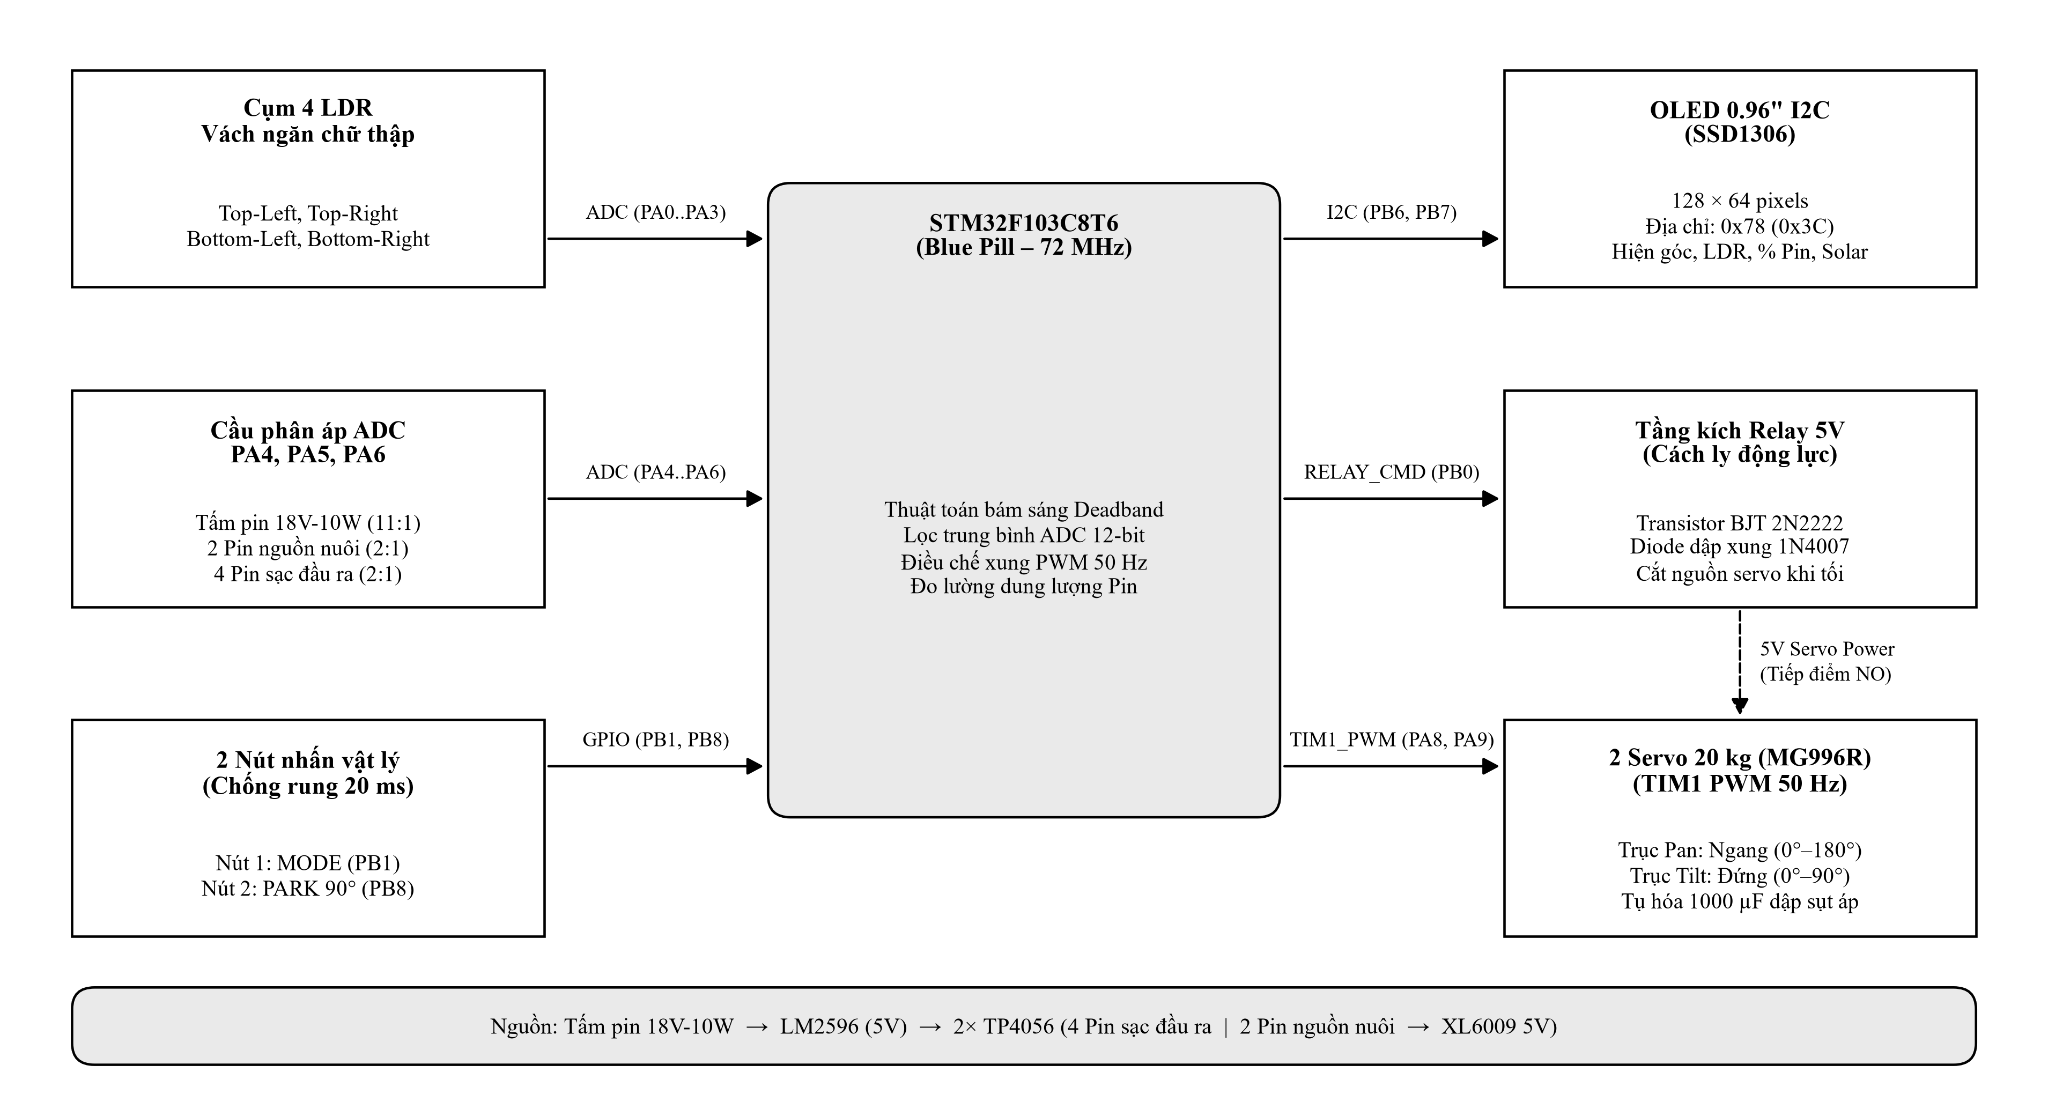
\includegraphics[width=0.92\textwidth,height=0.48\textheight,keepaspectratio]{images/img02_ch2_so_do_khoi.png}
  \caption{Sơ đồ khối hệ thống}
  \label{fig:img02}
\end{figure}

\subsection{Phân rã chức năng bậc một}

\textbf{F1 -- Thu nhận bức xạ \& Đo lường: }Đọc cường độ ánh sáng từ 4 cảm biến LDR (PA0..PA3) qua ADC 12-bit; đo điện áp phản hồi của khối 2 pin dự phòng (PA5), khối 4 pin lưu trữ (PA6) và điện áp tấm pin 18V (PA4).

\textbf{F2 -- Xử lý tín hiệu \& Bám sáng: }Lọc nhiễu trung bình 4 mẫu ADC; tính quang sai dH, dV; kiểm tra ngưỡng dung sai (Deadband tol = 25) chống rung lắc; đánh giá điều kiện ánh sáng Ngày/Đêm để bám sáng hoặc chuyển sang Sleep Mode.

\textbf{F3 -- Chấp hành cơ khí \& Cách ly: }Xuất 2 kênh xung PWM 50Hz độc lập điều khiển 2 Servo MG996R (20kg) cho trục Pan (0\textdegree{}--180\textdegree{}) và trục Tilt (0\textdegree{}--90\textdegree{}); điều khiển Relay 5V ngắt nguồn Servo khi trời không có nắng.

\textbf{F4 -- Biến đổi năng lượng \& Tích trữ: }Hạ áp LM2596 từ 18V xuống 5V, nạp dòng an toàn qua TP4056 cho khối 4 pin 18650 xả cao và khối 2 pin dự phòng logic; kích áp qua XL6009 cấp nguồn 5V ổn định.

\textbf{F5 -- Giao diện hiển thị: }Hiển thị \% pin và trạng thái hệ thống lên màn hình OLED 0.96" qua I2C; đưa vi điều khiển vào chế độ ngủ (Sleep Mode) khi tối và định kỳ thức dậy đo pin.

\section{Hardware Specification -- Đặc tả phần cứng}

Phần này mô tả chi tiết triển khai từng khối phần cứng, ánh xạ chân kết nối và mạch bảo vệ tạo nên hệ thống hoàn chỉnh.

\subsection{Vi điều khiển STM32F103C8T6 \& Bảng ánh xạ chân (Pinout)}

Bộ điều khiển trung tâm STM32F103C8T6 (ARM Cortex-M3 72MHz, 64KB Flash, 20KB SRAM, logic 3.3V, hỗ trợ chế độ ngủ tiết kiệm điện) sử dụng các chân sau:

{
\small
\setlength{\LTleft}{0pt}\setlength{\LTright}{0pt}
\begin{longtable}{>{\raggedright\arraybackslash}p{0.130\textwidth}>{\raggedright\arraybackslash}p{0.160\textwidth}>{\raggedright\arraybackslash}p{0.310\textwidth}>{\raggedright\arraybackslash}p{0.320\textwidth}}
\toprule
\textbf{Chân STM32} & \textbf{Ngoại vi} & \textbf{Kết nối phần cứng} & \textbf{Chức năng} \\
\midrule
\endfirsthead
\toprule
\textbf{Chân STM32} & \textbf{Ngoại vi} & \textbf{Kết nối phần cứng} & \textbf{Chức năng} \\
\midrule
\endhead
\bottomrule
\endfoot
\bottomrule
\endlastfoot
PA0 -- PA3 & ADC1\_IN0..3 & 4 cầu chia áp LDR (10k\ensuremath{\Omega}) & Đọc cường độ ánh sáng 4 góc (12-bit) \\
PA4 & ADC1\_IN4 & Cầu phân áp 100k\ensuremath{\Omega} / 10k\ensuremath{\Omega} (11:1) & Đo điện áp tấm pin 18V (22V \ensuremath{\to} 2.0V) \\
PA5 & ADC1\_IN5 & Cầu phân áp 10k\ensuremath{\Omega} / 10k\ensuremath{\Omega} (2:1) & Đo áp \& \% khối 2 pin dự phòng (4.2V \ensuremath{\to} 2.1V) \\
PA6 & ADC1\_IN6 & Cầu phân áp 10k\ensuremath{\Omega} / 10k\ensuremath{\Omega} (2:1) & Đo áp \& \% khối 4 pin lưu trữ (4.2V \ensuremath{\to} 2.1V) \\
PA8, PA9 & TIM1\_CH1/2 & 2 Servo MG996R (Pan, Tilt) & Xuất 2 kênh PWM 50Hz độc lập \\
PB0 & GPIO Output & Trở 1k\ensuremath{\Omega} \ensuremath{\to} BJT 2N2222 \ensuremath{\to} Relay 5V & Đóng/ngắt nguồn 2 Servo khi tối/mưa bão \\
PB6, PB7 & I2C1\_SCL/SDA & Màn hình OLED 0.96" (trở kéo 4.7k\ensuremath{\Omega}) & Truyền dữ liệu hiển thị \% pin \& trạng thái \\
\end{longtable}
}

\subsection{Cảm biến ánh sáng LDR}

\textbf{Cấu trúc bố trí: }Gồm 4 quang trở GL5528 bố trí đối xứng quanh vách ngăn chữ thập chắn sáng để phân biệt cường độ sáng theo hai phương ngang (Pan) và đứng (Tilt).

\textbf{Nguyên lý phần cứng: }Mỗi LDR mắc nối tiếp với 1 điện trở cố định 10k\ensuremath{\Omega} tạo mạch phân áp giữa +3.3V và GND; điện áp điểm giữa (0.2V--3.1V) đưa thẳng vào PA0..PA3 để ADC 12-bit chuyển đổi.

\subsection{Động cơ Servo MG996R (20kg)}

Sử dụng 2 động cơ Servo tải nặng MG996R (moment xoay 20 kg\ensuremath{\cdot}cm) để nâng và xoay ổn định mảng pin 34cm và khung cơ khí trọng lượng 2,0--2,5 kg:

\textbf{Servo Pan (PA8): }Điều chỉnh phương ngang trong dải 0\textdegree{}--180\textdegree{}.

\textbf{Servo Tilt (PA9): }Điều chỉnh phương đứng trong dải 0\textdegree{}--90\textdegree{}.

\textbf{Đặc tả điều khiển: }Điều khiển bằng 2 kênh PWM 50Hz độc lập từ TIM1, cấp nguồn riêng qua tiếp điểm Relay 5V và tụ bù để đáp ứng dòng khởi động đồng thời của cả 2 Servo.

\subsection{Tấm năng lượng mặt trời Waveshare 18V -- 10W}

Tấm quang điện đa tinh thể Waveshare 18V -- 10W (chiều dài 34 cm, điện áp danh định 18V), đóng vai trò nguồn thu chính cấp điện áp DC đầu vào cho khối hạ áp và sạc pin.

\subsection{Module hạ áp \& sạc pin (LM2596 \& TP4056)}

\textbf{Module giảm áp Buck LM2596: }Hạ áp từ 18V xuống chuẩn 5.0V (chịu dòng tối đa 3A) cấp cho tầng sạc.

\textbf{Module sạc Lithium TP4056 (2 mạch độc lập): }Quản lý dòng nạp CC/CV an toàn (1A, tự ngắt khi pin đạt 4.2V) cho khối 4 pin lưu trữ và khối 2 pin dự phòng.

\subsection{Module lưu trữ năng lượng (4 \texttimes{} 18650)}

Khối 4 cell pin Lithium-ion 18650 dòng xả cao mắc song song (3.7V danh định, 4.2V sạc đầy) làm khối tích trữ năng lượng chính thu từ mặt trời; điện áp khối pin được phản hồi qua cầu trở 10k\ensuremath{\Omega}/10k\ensuremath{\Omega} về chân PA6 để giám sát \% dung lượng.

\subsection{Module quản lý nguồn điện (XL6009 \& 2 \texttimes{} 18650 dự phòng)}

\textbf{Mạch tăng áp Boost XL6009: }Nâng điện áp pin (3.7V--4.2V) lên mức 5.0V ổn định cấp cho toàn hệ thống.

\textbf{Khối pin dự phòng logic (2 \texttimes{} 18650): }Cấp nguồn dự phòng cho STM32 và OLED khi không có ánh sáng mặt trời, duy trì khả năng định kỳ thức dậy giám sát pin, hiển thị thông số và ngủ an toàn vào ban đêm/thời tiết xấu.

\subsection{Module hiển thị (OLED 0.96" I2C)}

Màn hình OLED 0.96" (SSD1306, 128 \texttimes{} 64) giao tiếp I2C qua PB6/PB7 (địa chỉ 0x78), hiển thị \% dung lượng pin 18650 và trạng thái vận hành của hệ thống.

\subsection{Mạch cách ly động lực Relay 5V \& tụ chống sụt áp}

\textbf{Mạch kích \& bảo vệ Relay: }Chân PB0 điều khiển BJT NPN 2N2222 qua trở 1k\ensuremath{\Omega} (IB \ensuremath{\approx} 2.6mA) để đóng/ngắt cuộn hút Relay 5V (\ensuremath{\approx} 70mA); mắc song song ngược cực Diode 1N4007 dập xung cảm ứng bảo vệ BJT.

\textbf{Tụ hóa chống sụt áp 1000\ensuremath{\mu}F / 16V: }Tiếp điểm COM nối nguồn +5V, tiếp điểm NO cấp nguồn cho 2 Servo MG996R kèm tụ hóa 1000\ensuremath{\mu}F/16V mắc xuống GND để bù xung dòng đề-pa khi 2 Servo khởi động đồng thời, chống sụt áp reset STM32.

\begin{figure}[H]
  \centering
  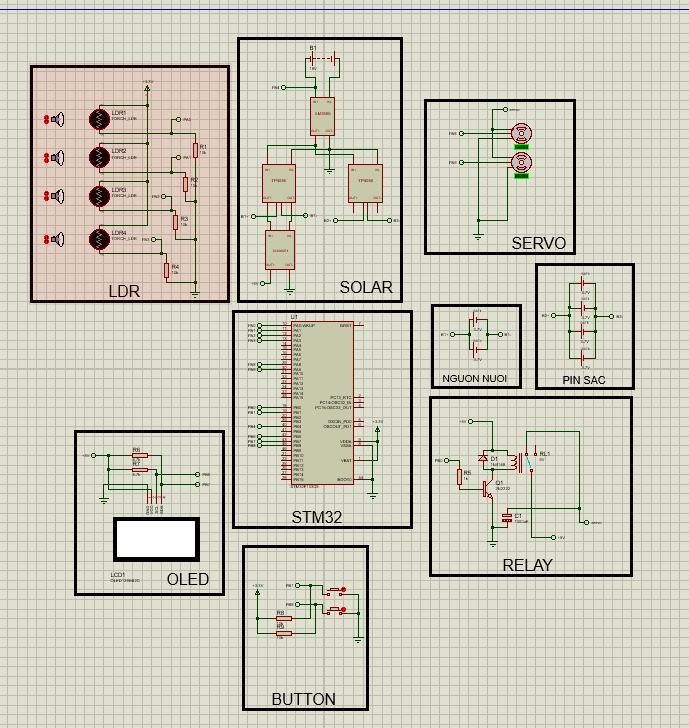
\includegraphics[width=0.92\textwidth,height=0.48\textheight,keepaspectratio]{images/img03_ch2_proteus_full.png}
  \caption{Sơ đồ nguyên lý phân chia khối chức năng trên phần mềm Proteus 8 (lưu ý bổ sung cầu trở PA4/PA5/PA6 và chỉnh đúng cực pin)}
  \label{fig:img03}
\end{figure}

\section{Software Specification -- Đặc tả phần mềm}

\subsection{External interfaces (Giao diện bên ngoài)}

\subsubsection*{4.1.1. Giao diện kết nối phần cứng }

Phần mềm nhúng trên vi điều khiển \textbf{STM32F103C8T6} giao tiếp trực tiếp với các ngoại vi phần cứng thông qua các chuẩn tín hiệu sau:

\textbf{Ngõ vào ADC 12-bit (5 kênh):}

\textbf{4 kênh:} Đọc tín hiệu điện áp tương tự từ 4 cảm biến quang trở (LDR) để xác định hướng nhận ánh sáng tối ưu nhất.

\textbf{2 kênh:} Đọc điện áp phản hồi độc lập từ 2 khối pin 18650 riêng biệt (1 kênh cho khối 4 pin lưu trữ sạc/output, 1 kênh cho khối 2 pin nguồn nuôi dự phòng hệ thống). 

\textbf{Ngõ ra PWM (2 kênh Timer độc lập):} Xuất xung điều khiển góc quay cho 2 động cơ Servo MG996R trên trục Pan () và trục Tilt ().

\textbf{Giao tiếp I2C:} Truyền dữ liệu phần trăm (\%) dung lượng pin sang màn hình hiển thị OLED.

\textbf{GPIO Output: }Mạch cách ly nguồn Servo (Relay  + tụ bù 1000uF) 

\textbf{GPIO Input (PB1) / Output (PC13): }Nút bấm MODE \& LED trạng thái 

\subsubsection*{4.1.2. Giao diện phần mềm}

Hệ thống được xây dựng theo kiến trúc bare-metal (không sử dụng hệ điều hành thời gian thực RTOS, không dùng bộ nhớ ngoài và không tích hợp cơ sở dữ liệu bên ngoài). Các giao diện phần mềm nội bộ bao gồm:

\textbf{Lớp truy cập phần cứng MCU:} Phần mềm ứng dụng (6 module: \textit{Sensor Processing, Sun Tracking Algorithm, Servo Control Algorithm, Battery Monitoring, Power Management, System Control}) giao tiếp với thanh ghi ngoại vi STM32F103C8T6 thông qua thư viện chuẩn STM32 HAL/LL Driver trên môi trường STM32Cube IDE. 

\textbf{Trình điều khiển đồ họa OLED:} Module hiển thị giao tiếp với thư viện điều khiển màn hình OLED (chuẩn SSD1306) thông qua vùng đệm khung hình Frame Buffer kích thước\textbf{ } cấp phát tĩnh trong bộ nhớ RAM nội. Dữ liệu chuỗi ký tự ASCII được định dạng vào Frame Buffer trước khi đẩy đồng bộ ra ngoại vi I2C. 

\subsection{Functions (Các yêu cầu chức năng)}

\subsubsection*{4.2.1. Chức năng 1 - Xử lý cảm biến và điều hướng bám sáng tự động 2 trục }

\textbf{a. Xử lý cảm biến }

\textbf{Thu thập và ánh xạ kênh ADC}: Định kỳ mỗi 1 giây (khi đủ nắng), đọc giá trị số hóa 12-bit từ 4 kênh ADC tương ứng với 4 cảm biến quang trở (LDR). Các kênh được ánh xạ cố định theo cấu hình bố trí vật lý thành 2 cặp đối xứng: cặp Trái -- Phải (tương ứng trục ngang Pan) và cặp Trên -- Dưới (tương ứng trục nghiêng Tilt). 

\textbf{Pha hiệu chuẩn cảm biến (Calibration Phase):} Thực hiện khi khởi động hệ thống tại vị trí lắp đặt thực tế (do hướng sáng môi trường và đặc tính phần cứng từng quang trở có sự sai lệch giữa các vị trí đặt). Phần mềm lấy mẫu giá trị ADC của 4 LDR trong điều kiện chiếu sáng nền tại chỗ để tính \textbf{giá trị bù lệch (Offset)} cho từng kênh và thiết lập ngưỡng \textbf{vùng dung sai (Deadband)} phù hợp. 

\textbf{b. Thuật toán bám sáng }

Tính toán mức độ chênh lệch ánh sáng (quang sai) từ 4 giá trị LDR đã chuẩn hóa theo từng trục bằng cách tổng hợp tín hiệu 2 cảm biến cùng phía: so sánh nửa Trái với nửa Phải cho trục ngang \textbf{Pan}, và nửa Trên với nửa Dưới cho trục nghiêng \textbf{Tilt}. 

\textbf{So sánh sai số với vùng dung sai}: 

Nếu quang sai nằm trong \textbf{vùng dung sai}, phần mềm giữ nguyên góc hiện tại để chống dao động liên tục (\textit{hunting}) gây lãng phí năng lượng. 

Nếu quang sai \textbf{vượt vùng dung sai}, phần mềm xác định chiều lệch và tính toán góc hiệu chỉnh để xoay bề mặt tấm pin vuông góc với hướng nắng (đảm bảo sai số định hướng ). 

\textbf{c. Điều khiển động cơ Servo (Servo Control) }

Xuất xung PWM độc lập qua Timer để điều khiển 2 động cơ Servo MG996R xoay trục Pan () và trục Tilt (). 

Đảm bảo điều khiển ổn định khi 2 động cơ khởi động đồng thời, không gây sụt áp làm reset vi điều khiển. 

\subsubsection*{4.2.2. Chức năng 2: Giám sát trạng thái và hiển thị dung lượng 2 khối Pin 18650 }

\textbf{Thu thập tín hiệu điện áp: }

Cấu hình 2 kênh ADC 12-bit (dải giá trị ) để đọc điện áp phản hồi độc lập từ khối 4 pin lưu trữ (output) và khối 2 pin nguồn dự phòng nuôi hệ thống.

Thực hiện đo điện áp theo chu kỳ hoạt động của hệ thống vào ban ngày và mỗi lần vi điều khiển thức dậy trong chế độ tiết kiệm điện (ban đêm hoặc thời tiết xấu). 

\textbf{Xử lý và quy đổi dung lượng: }

Chuyển đổi giá trị số hóa ADC của từng kênh sang mức điện áp thực tế tương ứng của mỗi khối pin. 

Ánh xạ giá trị điện áp đo được sang tỷ lệ phần trăm (\%) dung lượng riêng biệt cho khối 4 pin sạc và khối 2 pin nguồn nuôi. 

\textbf{Hiển thị thông số:} Đóng gói dữ liệu phần trăm (\%) dung lượng của cả 2 khối pin và truyền qua giao thức I2C để hiển thị rõ ràng lên màn hình OLED. 

\subsubsection*{4.2.3. Chức năng 3 - Quản lý nguồn điện (Ngủ đông và Khôi phục) }

\textbf{Kích hoạt chế độ ngủ (khi thiếu sáng):}

Khi cường độ ánh sáng từ 4 cảm biến quang trở (LDR) giảm xuống mức thấp (tương ứng điều kiện ban đêm hoặc mưa bão), hệ thống tự động ngắt nguồn ngoại vi (cụm 2 động cơ Servo) để quản trị dòng rò và đưa vi điều khiển STM32F103C8T6 vào chế độ ngủ.

Trong trạng thái này, hệ thống chuyển sang sử dụng khối 2 pin 18650 dự phòng làm nguồn nuôi logic riêng cho STM32 và màn hình OLED (chỉ kích hoạt khi không có ánh sáng mặt trời).

\textbf{Giám sát định kỳ trong lúc ngủ:}

Vi điều khiển định kỳ thức dậy (30 phút/lần) để đọc điện áp của 2 khối pin 18650, ánh xạ ra phần trăm và hiển thị lên màn hình OLED qua giao thức I2C.

Sau khi cập nhật thông số và kiểm tra ánh sáng vẫn chưa đạt ngưỡng hoạt động, phần mềm đưa vi điều khiển quay trở lại chế độ ngủ an toàn.

\textbf{Tự động khôi phục hoạt động: }Khi điều kiện ánh sáng đạt mức đủ nắng trở lại, hệ thống tự động đánh thức vi điều khiển, cấp nguồn lại cho ngoại vi và khôi phục chu trình điều hướng bám sáng

\subsubsection*{4.3.4. Sơ đồ khối thuật toán chức năng}

\begin{figure}[H]
  \centering
  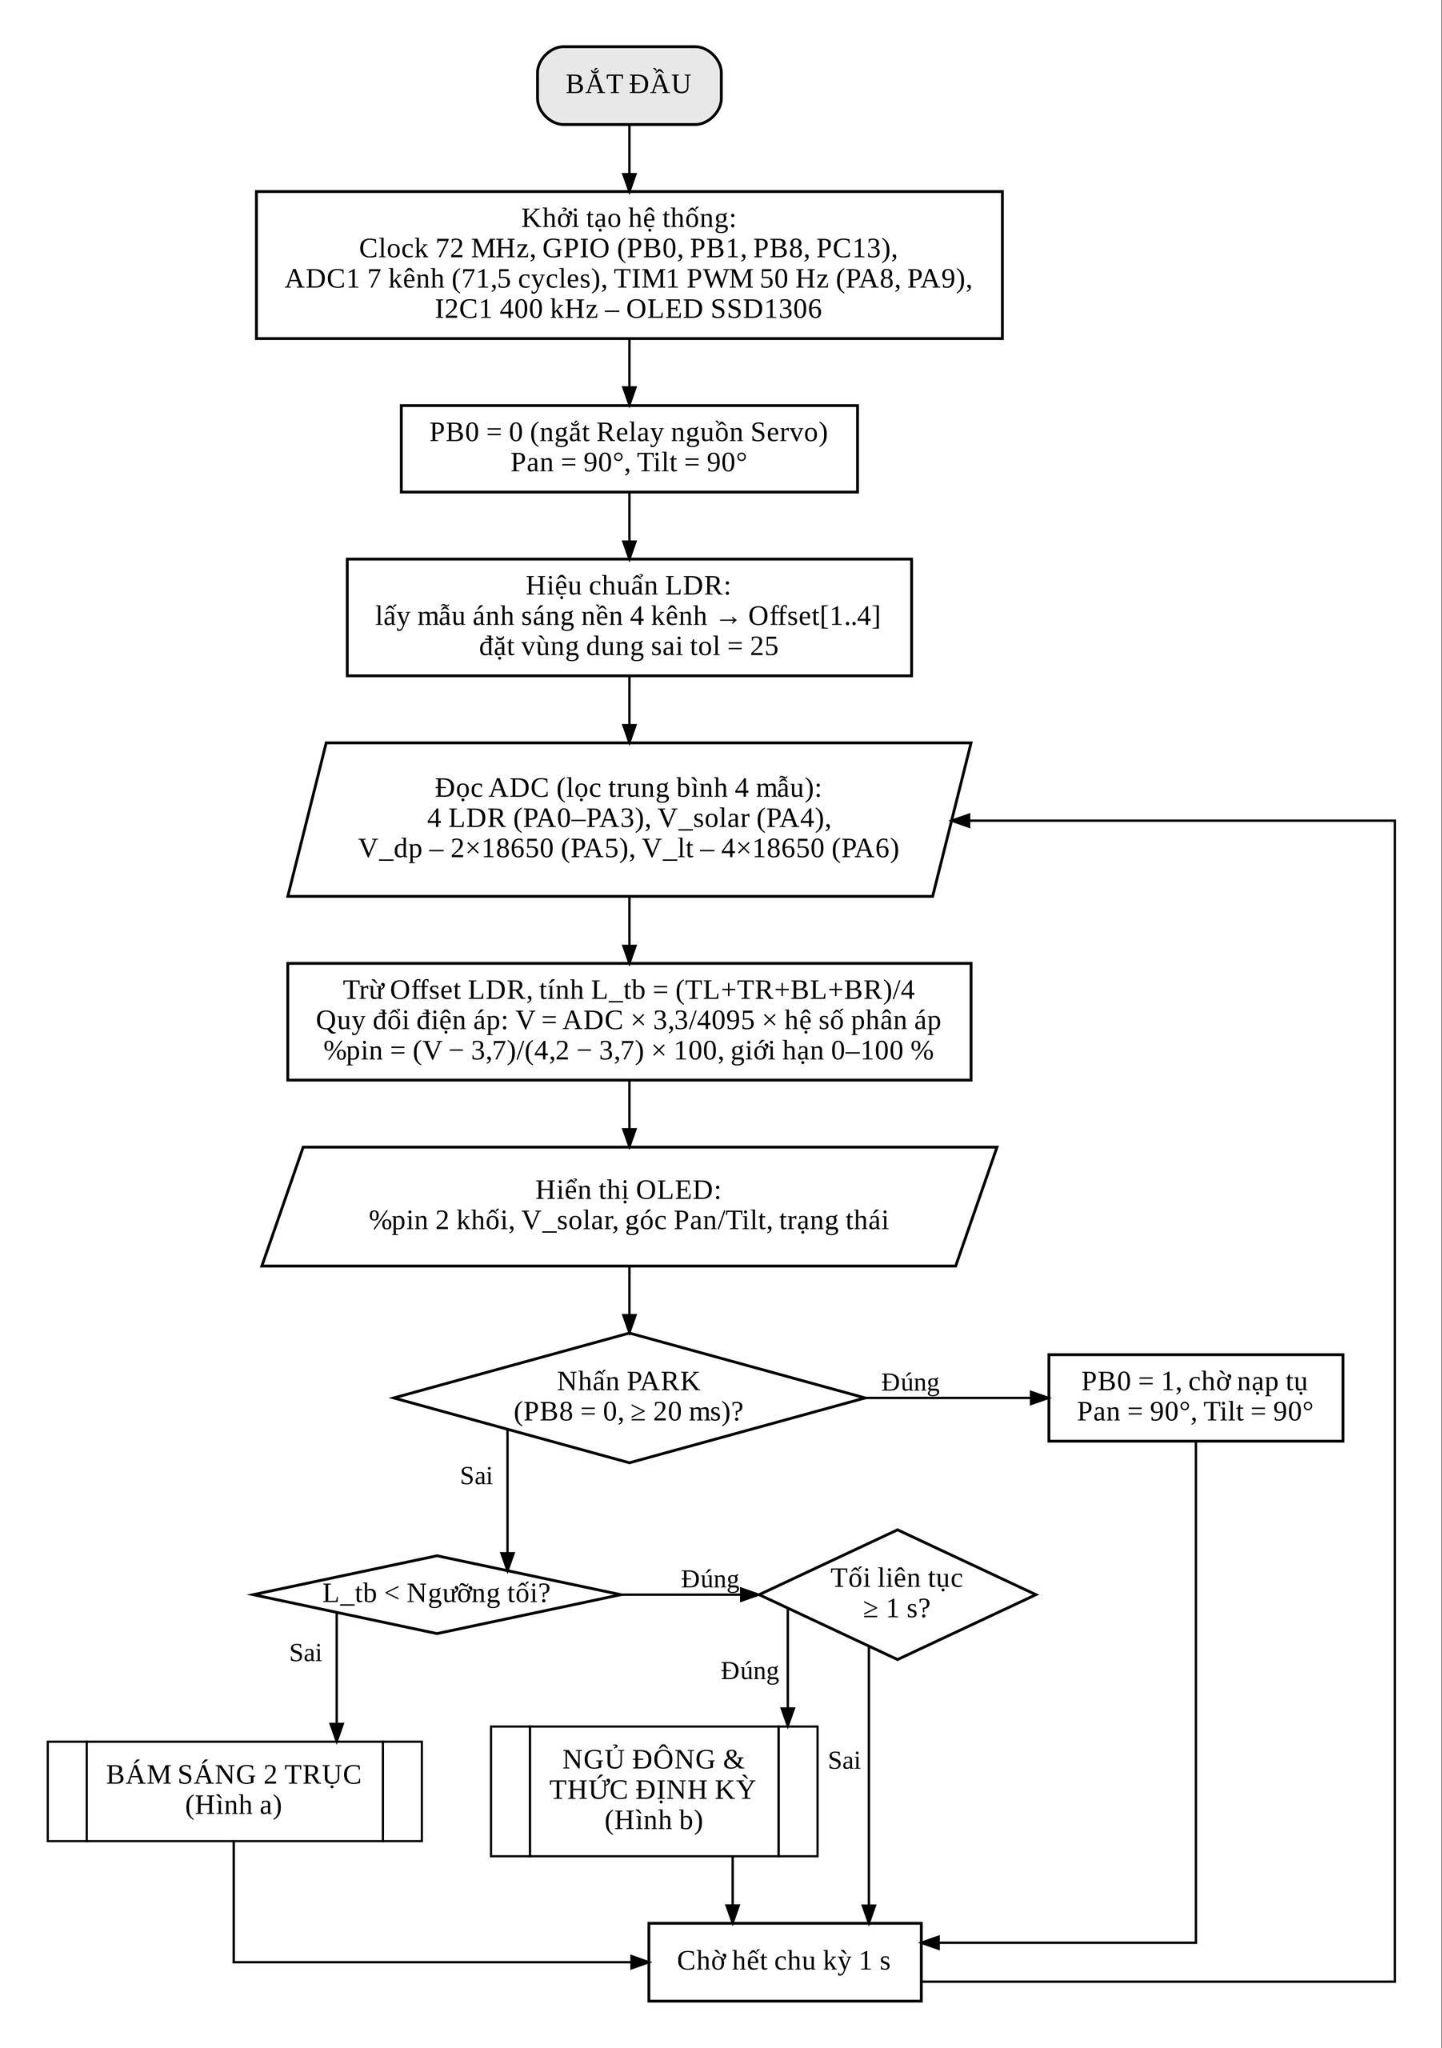
\includegraphics[height=0.72\textheight,width=\textwidth,keepaspectratio]{images/img04_ch2_luu_do_tong_quat.jpg}
  \caption{Lưu đồ tổng quát}
  \label{fig:img04}
\end{figure}

\begin{figure}[H]
  \centering
  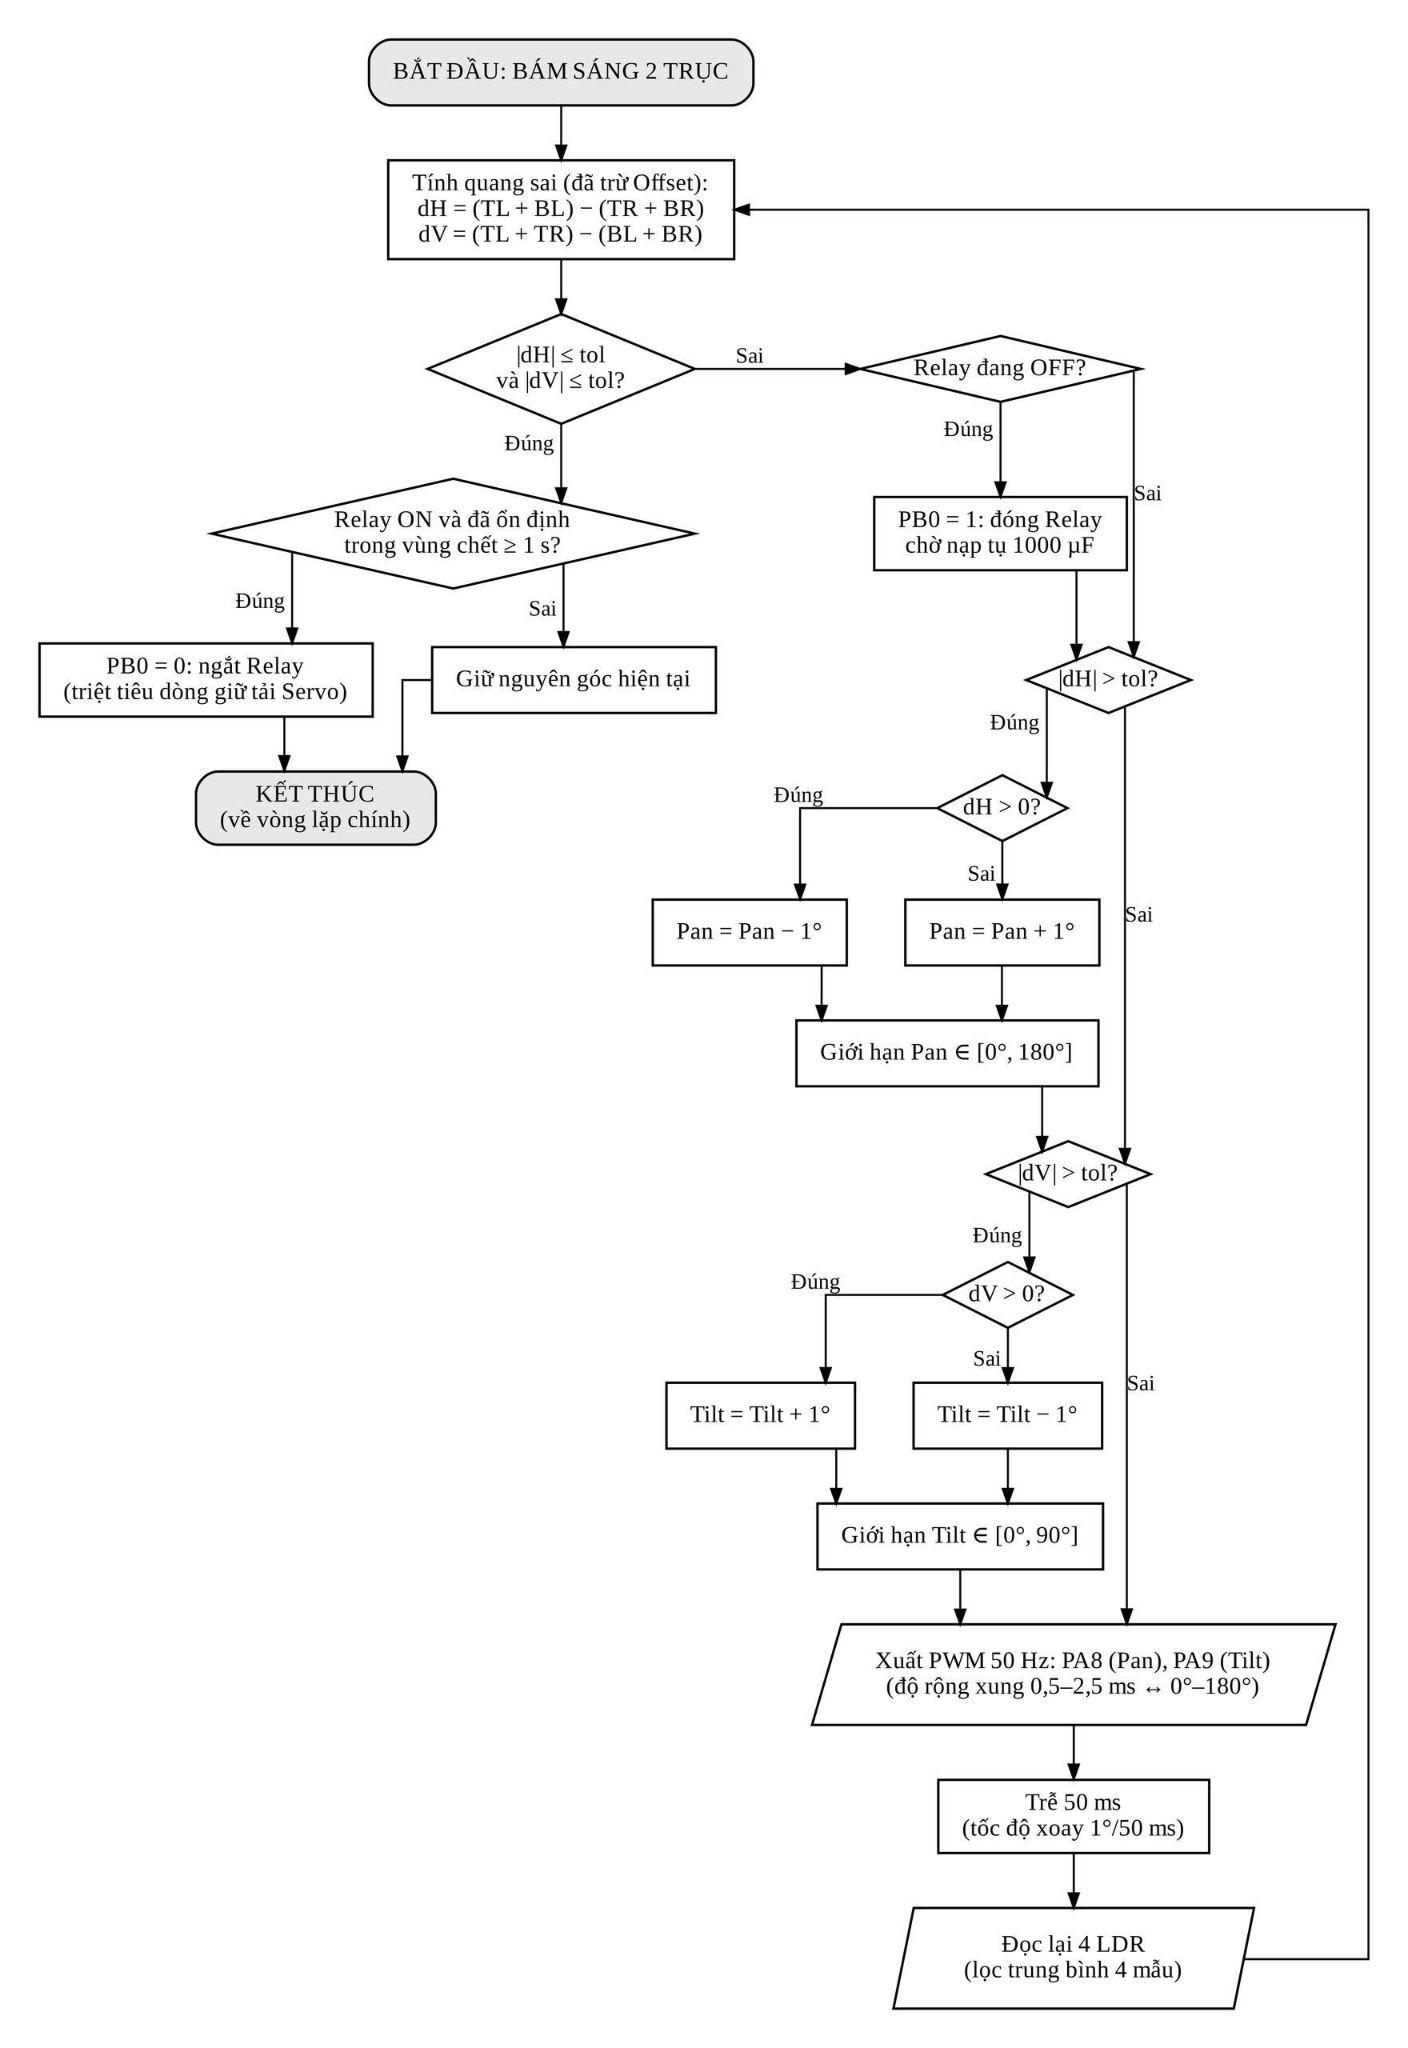
\includegraphics[height=0.72\textheight,width=\textwidth,keepaspectratio]{images/img05_ch2_luu_do_bam_sang.jpg}
  \caption{Lưu đồ giải thuật bám sáng}
  \label{fig:img05}
\end{figure}

\subsection{Yêu cầu về tính khả dụng (Usability Requirements)}

\textbf{Hiển thị trực quan:} Thông tin phần trăm (\%) dung lượng của cả khối 4 pin lưu trữ (output) và khối 2 pin nguồn nuôi dự phòng trên màn hình OLED phải được trình bày rõ ràng, phân biệt rạch ròi từng khối để người dùng dễ dàng theo dõi tình trạng tích trữ điện năng. 

\textbf{Vận hành tự động hoàn toàn:} Hệ thống hoạt động độc lập ngoài lưới; phần mềm tự động thực hiện hiệu chuẩn khi khởi động, bám sáng theo điều kiện nắng và chuyển đổi sang chế độ ngủ tiết kiệm điện vào ban đêm hoặc khi thời tiết xấu mà không yêu cầu bất kỳ thao tác điều khiển thủ công nào từ người dùng. 

\subsection{Yêu cầu về hiệu năng (Performance requirements).}

\textbf{Chu kỳ đáp ứng bám sáng:} Thời gian lấy mẫu tín hiệu từ 4 cảm biến quang trở (LDR) và cập nhật lệnh điều khiển bám sáng là định kỳ mỗi \textbf{1 giây}. 

\textbf{Phạm vi góc điều khiển:} Xung PWM xuất ra phải điều khiển chính xác toàn dải góc cơ học của 2 trục: \textbf{ }đến\textbf{ } đối với trục Pan và \textbf{ }đến\textbf{ } đối với trục Tilt. 

\textbf{Độ chính xác định hướng:} Sai số góc định hướng mục tiêu của mảng pin so với hướng ánh sáng mặt trời phải đạt . 

\textbf{Độ phân giải đo lường:} Dữ liệu từ 4 cảm biến LDR và điện áp phản hồi của 2 khối pin 18650 phải được số hóa qua bộ \textbf{ADC 12-bit}. 

\textbf{Khả năng chịu tải khi khởi động đồng thời:} Giải thuật xuất xung PWM điều khiển 2 động cơ Servo MG996R (momen xoắn ) phải đảm bảo vận hành ổn định, không gây sụt áp làm reset vi điều khiển STM32F103C8T6 khi 2 động cơ khởi động cùng lúc. 

\subsection{Design constraints (Ràng buộc thiết kế)}

\textbf{Ràng buộc điện áp vào MCU:} Điện áp tại tất cả các chân của STM32F103C8T6 không được vượt quá 3.3V; phần mềm phải tính toán dựa trên tỷ lệ cầu phân áp đã hạ điện áp hở mạch 18V của tấm pin xuống dải 0 - 2.0V.

\textbf{An toàn pin Lithium và module:} Giám sát và ánh xạ dung lượng pin 18650 trong ngưỡng điện áp an toàn 3.7 - 4.2V. Phần mềm phối hợp với phần cứng cách ly nguồn Servo (Relay  + tụ bù 1000uF) thông qua trễ nạp tụ để ngăn sụt áp gây reset MCU. Việc vận hành phần mềm phải tương thích với giới hạn phần cứng của mạch hạ áp LM2596 (), mạch sạc TP4056 ( CC/CV), mạch tăng áp XL6009 (công suất đỉnh < 12.5W). 

\subsection{Software system attributes (Thuộc tính hệ thống phần mềm)}

\textbf{Độ tin cậy:} Hệ thống có thể vận hành liên tục 24/7 mà không bị treo hoặc reset ngoài ý muốn nhờ cơ chế lọc nhiễu 4 mẫu, giới hạn tốc độ xoay , độ trễ nạp tụ và tín hiệu giám sát LED.

\textbf{Tính ổn định trước nhiễu môi trường:} Vùng chết tol = 25 triệt tiêu dao động quanh vị trí cân bằng; độ trễ ngắt Relay  giúp hệ thống không tắt nhầm động cơ khi có bóng mây hoặc vật thể lướt nhanh qua cảm biến. 

\textbf{Khả năng khắc phục sự cố:} Mã nguồn được chia tách rõ ràng thành 6 module chức năng độc lập (Sensor Processing, Sun Tracking, Servo Control, Battery Monitoring, Power Management, System Control) và tập trung toàn bộ hằng số hiệu chỉnh và kiểm thử từng phần. 

\section{Test Hardware Specification -- Đặc tả kiểm thử phần cứng}

{
\small
\setlength{\LTleft}{0pt}\setlength{\LTright}{0pt}
\begin{longtable}{>{\raggedright\arraybackslash}p{0.190\textwidth}>{\raggedright\arraybackslash}p{0.340\textwidth}>{\raggedright\arraybackslash}p{0.390\textwidth}}
\toprule
\textbf{Module kiểm thử} & \textbf{Phương pháp kiểm tra} & \textbf{Kết quả mong đợi (Định lượng)} \\
\midrule
\endfirsthead
\toprule
\textbf{Module kiểm thử} & \textbf{Phương pháp kiểm tra} & \textbf{Kết quả mong đợi (Định lượng)} \\
\midrule
\endhead
\bottomrule
\endfoot
\bottomrule
\endlastfoot
STM32F103C8T6 & Cấp nguồn 5V vào bo, kiểm tra áp nội 3.3V và LED trạng thái PC13. & Điện áp logic đạt 3.3V \textpm{} 0.05V, chip khởi động ổn định, vào/thoát Sleep Mode đúng chu kỳ. \\
Cụm 4 LDR & Chiếu đèn pin lần lượt vào từng quang trở và đo điện áp tại PA0..PA3. & Điện áp thay đổi tuyến tính trong dải 0.2V--3.1V theo độ sáng, giá trị ADC 12-bit (0--4095) ổn định. \\
Cầu phân áp đo áp & Cấp áp chuẩn 18V (Solar) và 4.2V (Pin), đo áp tại PA4, PA5, PA6. & PA4 \ensuremath{\approx} 1.64V (tối đa 2.0V ở 22V); PA5, PA6 \ensuremath{\approx} 2.10V ở 4.2V (luôn \ensuremath{\le} 3.3V). \\
2 Servo MG996R & Xuất xung PWM 50Hz độc lập trên PA8, PA9 kiểm tra toàn dải góc. & Trục Pan xoay đúng 0\textdegree{}--180\textdegree{}, trục Tilt xoay đúng 0\textdegree{}--90\textdegree{}, sai số góc \ensuremath{\le} \textpm{}5\textdegree{}. \\
Relay 5V \& Tụ 1000\ensuremath{\mu}F & Kích PB0 = 0/1 và cho 2 Servo MG996R khởi động đồng thời; đo áp bus 5V. & PB0 = 0 cắt nguồn Servo về 0V; PB0 = 1 cấp đủ 5V; áp bus 5V không tụt dưới 4.75V, STM32 không reset. \\
LM2596 & Cấp 18V từ tấm pin / nguồn DC vào IN+/IN-, đo áp ngõ ra OUT+/OUT-. & Điện áp ngõ ra đạt chuẩn 5.0V \textpm{} 0.1V ổn định khi có tải sạc. \\
TP4056 & Cấp 5V vào IN+/IN- sạc cho khối pin 18650, theo dõi đèn báo và điện áp pin. & Đèn đỏ sáng khi đang sạc (\ensuremath{\approx} 1A), tự chuyển xanh và ngắt sạc khi pin đạt 4.2V \textpm{} 0.05V. \\
XL6009 & Cấp nguồn từ khối pin 18650 (3.7V--4.2V) vào ngõ vào, đo ngõ ra có tải. & Điện áp ngõ ra tăng ổn định đạt 5.0V \textpm{} 0.1V. \\
Pin 18650 & Đo điện áp hở mạch và khi có tải của khối 4 pin lưu trữ \& khối 2 pin dự phòng. & Điện áp nằm trong giới hạn an toàn 3.0V--4.2V; khối 2 pin dự phòng nuôi STM32 \& OLED ổn định khi rút nguồn Solar. \\
OLED 0.96" I2C & Gửi dữ liệu mẫu qua PB6/PB7 (400kHz, địa chỉ 0x78). & Hiển thị rõ nét \% pin, góc quay và trạng thái hệ thống, không sọc hình hay treo bus I2C. \\
\end{longtable}
}

\chapter{THIẾT KẾ PHẦN CỨNG (HARDWARE DESIGN)}

\section{Thiết kế Sơ đồ khối Phần cứng (Hardware Block Diagram)}

\subsection{Phân tích thành phần phần cứng (Hardware Components)}

Hệ thống tích trữ năng lượng mặt trời tích hợp bám sáng tự động bao gồm 7 khối phần cứng chính và 1 khối bổ trợ phục vụ giám sát điện áp --- thao tác trực tiếp trên mô hình Proteus:

{
\small
\setlength{\LTleft}{0pt}\setlength{\LTright}{0pt}
\begin{longtable}{>{\raggedright\arraybackslash}p{0.060\textwidth}>{\raggedright\arraybackslash}p{0.220\textwidth}>{\raggedright\arraybackslash}p{0.260\textwidth}>{\raggedright\arraybackslash}p{0.380\textwidth}}
\toprule
\textbf{STT} & \textbf{Tên khối chức năng} & \textbf{Thành phần chính} & \textbf{Nhiệm vụ \& Thông số đặc tả} \\
\midrule
\endfirsthead
\toprule
\textbf{STT} & \textbf{Tên khối chức năng} & \textbf{Thành phần chính} & \textbf{Nhiệm vụ \& Thông số đặc tả} \\
\midrule
\endhead
\bottomrule
\endfoot
\bottomrule
\endlastfoot
1 & \textbf{Khối thu năng lượng mặt trời} & Tấm pin Waveshare 18V-10W & Tấm pin đa tinh thể, kích thước cạnh xấp xỉ 34cm, chuyển đổi quang năng thành điện áp danh định 18V cấp cho khối hạ áp và sạc lưu trữ. \\
2 & \textbf{Khối cảm biến quang \& Vách ngăn} & 4\texttimes{} LDR GL5528 + 4\texttimes{} 10k\ensuremath{\Omega} & Bố trí 4 góc (Top-Left, Top-Right, Bottom-Left, Bottom-Right) sau vách ngăn chữ thập tạo độ chênh lệch ánh sáng giữa 4 hướng; chuyển đổi cường độ sáng thành điện áp đưa về ADC 12-bit (PA0..PA3). \\
3 & \textbf{Khối vi điều khiển trung tâm} & STM32F103C8T6 (Blue Pill) & Lõi ARM Cortex-M3 32-bit, xung nhịp 72MHz, logic 3.3V; lọc trung bình ADC, tính sai lệch bám sáng (\textit{Deadband}), phát xung PWM 50Hz, kích Relay và truyền hiển thị I2C. \\
4 & \textbf{Khối nguồn \& Lưu trữ năng lượng} & LM2596, 2\texttimes{} TP4056, XL6009, 4x 18650, 2x 18650 & Hạ áp 18V\ensuremath{\to}5V (LM2596); sạc CC/CV 1A (2x TP4056): 4x 18650 làm pin sạc lưu trữ đầu ra (Output độc lập) và 2x 18650 làm nguồn nuôi nội bộ nối qua XL6009 nâng áp +5V cấp toàn hệ thống. \\
5 & \textbf{Khối kích Relay cách ly động lực} & Relay 5V, 2N2222, 1N4007, 1000\ensuremath{\mu}F/16V & Nhận lệnh từ PB0 (STM32) đóng/ngắt nguồn 5V cấp cho hai Servo, triệt tiêu dòng tĩnh ban đêm và dập xung sụt áp khởi động bằng tụ hóa 1000\ensuremath{\mu}F. \\
6 & \textbf{Khối cơ cấu chấp hành bám sáng} & 2\texttimes{} Servo MG996R (20 kg\ensuremath{\cdot}cm) & Cơ cấu 2 trục Pan-Tilt mang tấm pin 34cm: trục Pan quay ngang 0\textdegree{}--180\textdegree{} (PA8), trục Tilt ngẩng dọc 0\textdegree{}--90\textdegree{} (PA9), đảm bảo sai số bám sáng \ensuremath{\le} \textpm{}5\textdegree{}. \\
7 & \textbf{Khối hiển thị thông số} & OLED 0.96" I2C (SSD1306) & Độ phân giải 128\texttimes{}64 pixels, giao tiếp I2C1 (PB6/PB7, 400 kHz, địa chỉ 0x3C / 0x78), hiển thị góc Pan/Tilt, giá trị LDR, \% Pin và điện áp Solar. \\
8 & \textbf{Khối bổ trợ Proteus (Giám sát \& Nút nhấn)} & 3 cầu phân áp ADC + 2 nút nhấn & Cầu phân áp PA4 (100k\ensuremath{\Omega}/10k\ensuremath{\Omega}) đo áp Solar 18V, PA5 (10k\ensuremath{\Omega}/10k\ensuremath{\Omega}) đo 2x 18650 nguồn nuôi, PA6 (10k\ensuremath{\Omega}/10k\ensuremath{\Omega}) đo 4x 18650 pin sạc đầu ra; nút MODE (PB1) và PARK 90\textdegree{} (PB8). \\
\end{longtable}
}

\subsection{Sơ đồ khối phần cứng tổng thể}

Sơ đồ khối phần cứng hệ thống được trình bày tại \textbf{Hình 1}. Sơ đồ thể hiện rõ hai hướng luồng vật lý: luồng tín hiệu đo lường --- điều khiển xung quanh vi điều khiển STM32F103C8T6 và luồng năng lượng từ tấm pin 18V-10W qua các tầng biến đổi nguồn tới hai cụm pin 18650 và tải động cơ.

\begin{figure}[H]
  \centering
  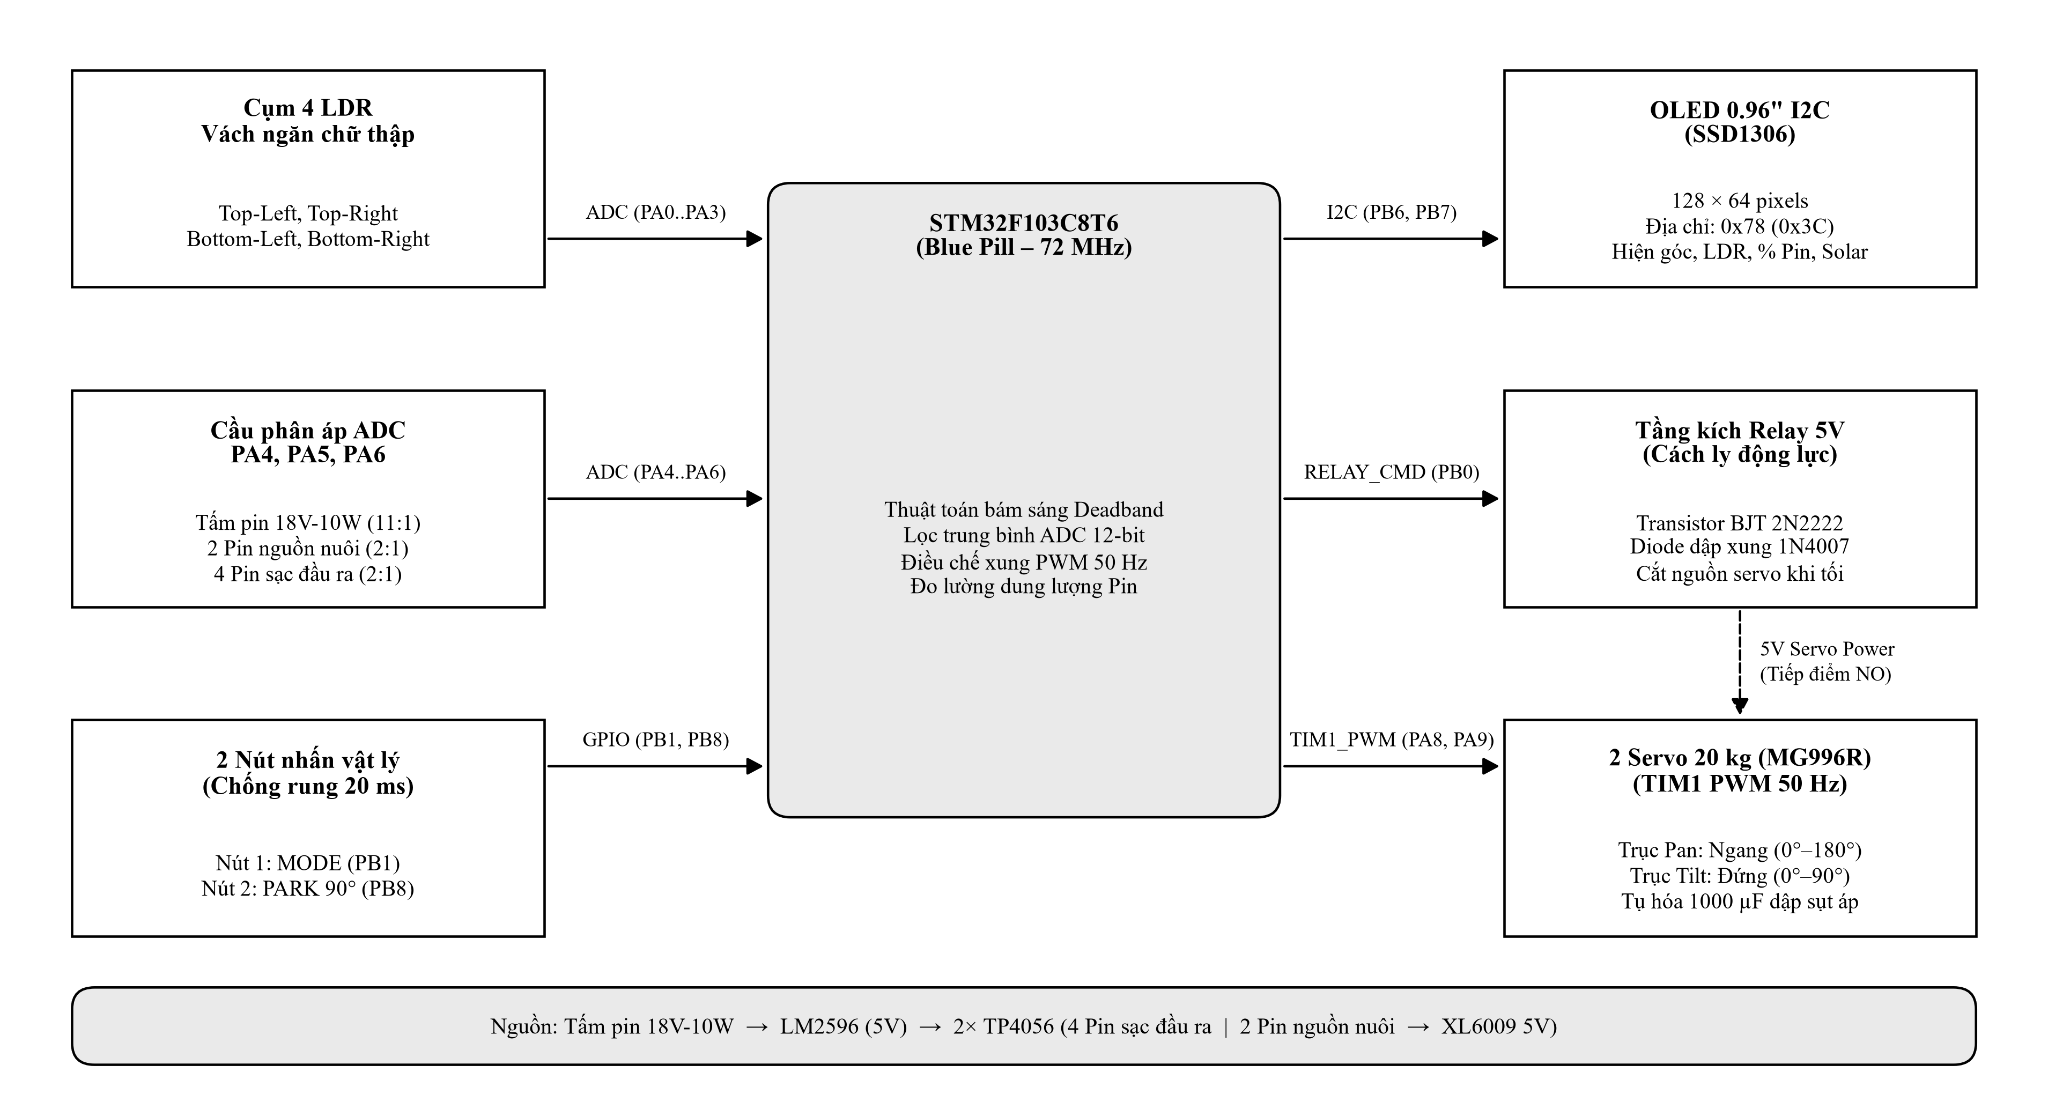
\includegraphics[width=0.92\textwidth,height=0.48\textheight,keepaspectratio]{images/img06_ch3_so_do_khoi.png}
  \caption{Sơ đồ khối phần cứng hệ thống Solar Tracker.}
  \label{fig:img06}
\end{figure}

\subsection{Luồng tín hiệu, dữ liệu và giao tiếp trên bo mạch}

\textbf{Luồng thu thập tín hiệu tương tự :} Bốn cầu phân áp từ cụm LDR GL5528 (PA0..PA3) và ba cầu phân áp bổ trợ đo điện áp nguồn (PA4..PA6) đi qua dây tín hiệu tương tự ngắn về bộ ADC 12-bit của STM32F103C8T6.

\textbf{Luồng điều khiển chấp hành :} Vi điều khiển xuất tín hiệu điều khiển số tại PB0 (RELAY\_CMD) kích đóng nguồn 5V qua tiếp điểm NO của Relay 5V, sau đó xuất hai kênh xung TIM1\_PWM 50Hz tại PA8 (Pan) và PA9 (Tilt) dẫn tới hai động cơ MG996R.

\textbf{Giao tiếp nội bộ :} Màn hình OLED SSD1306 giao tiếp qua bus I2C1 chuẩn hai dây (PB6 - SCL, PB7 - SDA) dùng chung hai điện trở kéo lên 4.7k\ensuremath{\Omega}; hai nút nhấn vật lý PB1 và PB8 nối trực tiếp về GPIO ngõ vào tích hợp điện trở kéo lên 10k\ensuremath{\Omega}.

\section{Lựa chọn Vi điều khiển}

\subsection{Thống kê yêu cầu I/O tối thiểu (Minimum I/O Requirements)}

Bảng dưới đây liệt kê toàn bộ chân giao tiếp cần thiết để vận hành đồng thời hệ thống bám sáng, quản lý nguồn và phần bổ trợ trên sơ đồ nguyên lý:

{
\small
\setlength{\LTleft}{0pt}\setlength{\LTright}{0pt}
\begin{longtable}{>{\raggedright\arraybackslash}p{0.180\textwidth}>{\raggedright\arraybackslash}p{0.190\textwidth}>{\raggedright\arraybackslash}p{0.080\textwidth}>{\raggedright\arraybackslash}p{0.290\textwidth}>{\raggedright\arraybackslash}p{0.180\textwidth}}
\toprule
\textbf{Nhóm ngoại vi} & \textbf{Kênh / Chân trên STM32} & \textbf{Số chân} & \textbf{Chức năng chi tiết} & \textbf{Chế độ cấu hình} \\
\midrule
\endfirsthead
\toprule
\textbf{Nhóm ngoại vi} & \textbf{Kênh / Chân trên STM32} & \textbf{Số chân} & \textbf{Chức năng chi tiết} & \textbf{Chế độ cấu hình} \\
\midrule
\endhead
\bottomrule
\endfoot
\bottomrule
\endlastfoot
\textbf{ADC 12-bit (Chính)} & PA0, PA1, PA2, PA3 & 4 & Đọc điện áp cầu phân áp 4\texttimes{} LDR GL5528 (TL, TR, BL, BR) & Analog Input \\
\textbf{ADC 12-bit (Bổ trợ)} & PA4, PA5, PA6 & 3 & Đo áp tấm pin 18V-10W (11:1), 2x 18650 nguồn nuôi (2:1), 4x 18650 đầu ra (2:1) & Analog Input \\
\textbf{TIM1 PWM 50Hz} & PA8 (CH1), PA9 (CH2) & 2 & Xuất xung PWM điều khiển Pan Servo (0\textdegree{}--180\textdegree{}) và Tilt Servo (0\textdegree{}--90\textdegree{}) & AF Push-Pull \\
\textbf{I2C1 Bus} & PB6 (SCL), PB7 (SDA) & 2 & Giao tiếp màn hình OLED 0.96" SSD1306 (0x3C / 0x78, 400 kHz) & AF Open-Drain \\
\textbf{GPIO Output} & PB0 (RELAY\_CMD) & 1 & Xuất mức logic 3.3V kích BJT 2N2222 đóng Relay 5V cấp Servo & Output Push-Pull \\
\textbf{GPIO Input (Bổ trợ)} & PB1 (MODE), PB8 (PARK) & 2 & Đọc 2 nút nhấn vật lý chuyển chế độ và đưa về góc an toàn 90\textdegree{} & Input (Pull-up 10k\ensuremath{\Omega}) \\
\textbf{Debug / Nạp code} & PA13 (SWDIO), PA14 (SWCLK) & 2 & Giao tiếp mạch nạp và gỡ lỗi phần cứng thời gian thực ST-Link V2 & SWD Interface \\
\midrule
\textbf{Tổng cộng} & \textbf{---} & \textbf{16} & \textbf{Đáp ứng hoàn toàn trên vỏ chân LQFP48 (37 GPIO khả dụng)} & \textbf{Còn dư 21 GPIO} \\
\end{longtable}
}

\subsection{Đánh giá 5 tiêu chí kỹ thuật lựa chọn STM32F103C8T6}

\textbf{1. Đáp ứng I/O tối thiểu:} Tổng nhu cầu sử dụng \textbf{7 kênh ADC}, \textbf{2 kênh PWM phần cứng}, \textbf{1 cổng I2C} và \textbf{3 chân GPIO}. STM32F103C8T6 tích hợp 2 bộ ADC 12-bit độc lập (tối đa 10 kênh ngoại vi trên gói 48 chân), 4 bộ định thời (TIM1 tạo xung PWM 50Hz độ phân giải cao) và 2 bộ I2C phần cứng, đáp ứng đầy đủ mà không cần mở rộng IC bên ngoài.

\textbf{2. Kiến trúc 32-bit (ARM Cortex-M3 72MHz):} Xử lý nhanh phép lọc trung bình động (\textit{Moving Average}) trên 7 kênh ADC 12-bit, phép tính chênh lệch 4 góc LDR kèm vùng trễ \textit{Deadband} (\ensuremath{\le} \textpm{}5\textdegree{}) và ước lượng phần trăm pin theo điện áp mà không làm trễ chu kỳ điều chế xung 20 ms.

\textbf{3. Nhu cầu bộ nhớ (64KB Flash / 20 KB SRAM):} Trình điều khiển OLED SSD1306 (128\texttimes{}64) cần bộ đệm hiển thị (128 \texttimes{} 64 / 8 = 1024 bytes RAM), cộng thêm các biến lọc ADC và thư viện HAL . Với 20 KB SRAM và 64KB Flash, hệ thống dư trên 50\% tài nguyên, tránh tình trạng tràn RAM như các dòng 8-bit (ATmega328P chỉ có 2 KB SRAM).

\textbf{4. Chi phí và tiêu thụ năng lượng thấp (Cost \& Low Power):} Kit phát triển Blue Pill STM32F103C8T6 có giá thành rất hợp lý (\textasciitilde{}65.000 VNĐ), hoạt động ở mức áp logic 3.3V (2.0V--3.6V) và hỗ trợ chế độ ngủ tiết kiệm điện (\textbf{Stop Mode}), giúp giảm đáng kể dòng tiêu thụ vào ban đêm khi nuôi bằng khối pin nguồn 2x 18650.

\textbf{5. Tính sẵn có và hệ sinh thái phát triển:} Linh kiện sẵn có tại thị trường Việt Nam, được hỗ trợ đồng bộ bởi phần mềm STM32Cube IDE, mạch nạp/gỡ lỗi ST-Link V2 và thư viện mô phỏng sẵn trong Proteus 8.

\subsection{So sánh nhanh các phương án vi điều khiển ứng viên}

{
\small
\setlength{\LTleft}{0pt}\setlength{\LTright}{0pt}
\begin{longtable}{>{\raggedright\arraybackslash}p{0.190\textwidth}>{\raggedright\arraybackslash}p{0.250\textwidth}>{\raggedright\arraybackslash}p{0.240\textwidth}>{\raggedright\arraybackslash}p{0.240\textwidth}}
\toprule
\textbf{Tiêu chí so sánh} & \textbf{STM32F103C8T6 (Được chọn)} & \textbf{ATmega328P (Arduino Uno/Nano)} & \textbf{ESP32-WROOM-32} \\
\midrule
\endfirsthead
\toprule
\textbf{Tiêu chí so sánh} & \textbf{STM32F103C8T6 (Được chọn)} & \textbf{ATmega328P (Arduino Uno/Nano)} & \textbf{ESP32-WROOM-32} \\
\midrule
\endhead
\bottomrule
\endfoot
\bottomrule
\endlastfoot
\textbf{Kiến trúc \& Xung nhịp} & ARM Cortex-M3 32-bit, 72 MHz & AVR 8-bit, 16 MHz & Xtensa LX6 32-bit, 240 MHz \\
\textbf{Bộ nhớ Flash / SRAM} & 64 KB / 20 KB & 32 KB / 2 KB (hạn hẹp cho OLED) & 4 MB / 520 KB \\
\textbf{Độ phân giải ADC} & \textbf{12-bit} (4096 mức, 10 kênh) & 10-bit (1024 mức, 8 kênh) & 12-bit (phi tuyến mạnh ở hai đầu dải) \\
\textbf{Tiêu thụ năng lượng} & Thấp (3.3V, hỗ trợ Stop Mode tốt) & Trung bình (5V) & Cao (thu phát Wi-Fi không dùng gây hao pin) \\
\textbf{Mức độ phù hợp dự án} & \textbf{Tối ưu} (chính xác cao, đủ RAM, tiết kiệm pin) & Độ phân giải thấp hơn, thiếu RAM & Dư thừa kết nối không dây, tốn pin dự phòng \\
\end{longtable}
}

\section{Thiết kế Nguồn và Quản lý Pin (Power Tree \& Battery Design)}

\subsection{Lựa chọn bộ biến đổi DC-DC so với ổn áp tuyến tính}

\textbf{Phân tích loại bỏ ổn áp tuyến tính (7805):} Nếu hạ áp trực tiếp từ tấm pin 18V xuống 5V bằng IC tuyến tính LM7805, hiệu suất chuyển đổi chỉ đạt mức rất thấp:

\textit{\ensuremath{\eta}\_7805 \ensuremath{\approx} V\_out / V\_in = 5V / 18V \ensuremath{\approx} 27.8\%   }

Với tấm pin công suất 10W, việc tiêu tán phần lớn công suất thành nhiệt trên ổn áp tuyến tính vừa gây quá nhiệt linh kiện vừa không đủ dòng để sạc pin và cấp cho cơ cấu quay.

\textbf{Lựa chọn mạch hạ áp xung LM2596 (Buck Converter):} Hoạt động ở tần số đóng cắt 150 kHz với hiệu suất cao (\ensuremath{\approx} 80\% -- 88\%), dòng tải tối đa 3A. Mạch hạ điện áp từ tấm pin 18V-10W xuống bus ổn áp chuẩn 5.0V cấp đồng thời cho hai module sạc pin TP4056.

\textbf{Lựa chọn mạch tăng áp xung XL6009 (Boost Converter):} Khối nguồn nuôi \textbf{2x 18650} có điện áp biến thiên trong dải 3.0V -- 4.2V. Bộ XL6009 được nối trực tiếp từ khối 2x 18650 để nâng ổn định lên đường bus \textbf{+5.0V hệ thống}, cấp nguồn đồng thời cho hai nhánh: nhánh động lực 2x Servo MG996R (qua tiếp điểm Relay 5V) và kit STM32 Blue Pill (qua LDO nội hạ xuống 3.3V cấp cho STM32, OLED, LDR, nút nhấn).

\subsection{Cấu trúc Cây nguồn (Power Tree) --- Phân tách Đầu ra và Nhánh nuôi Hệ thống}

\begin{figure}[H]
  \centering
  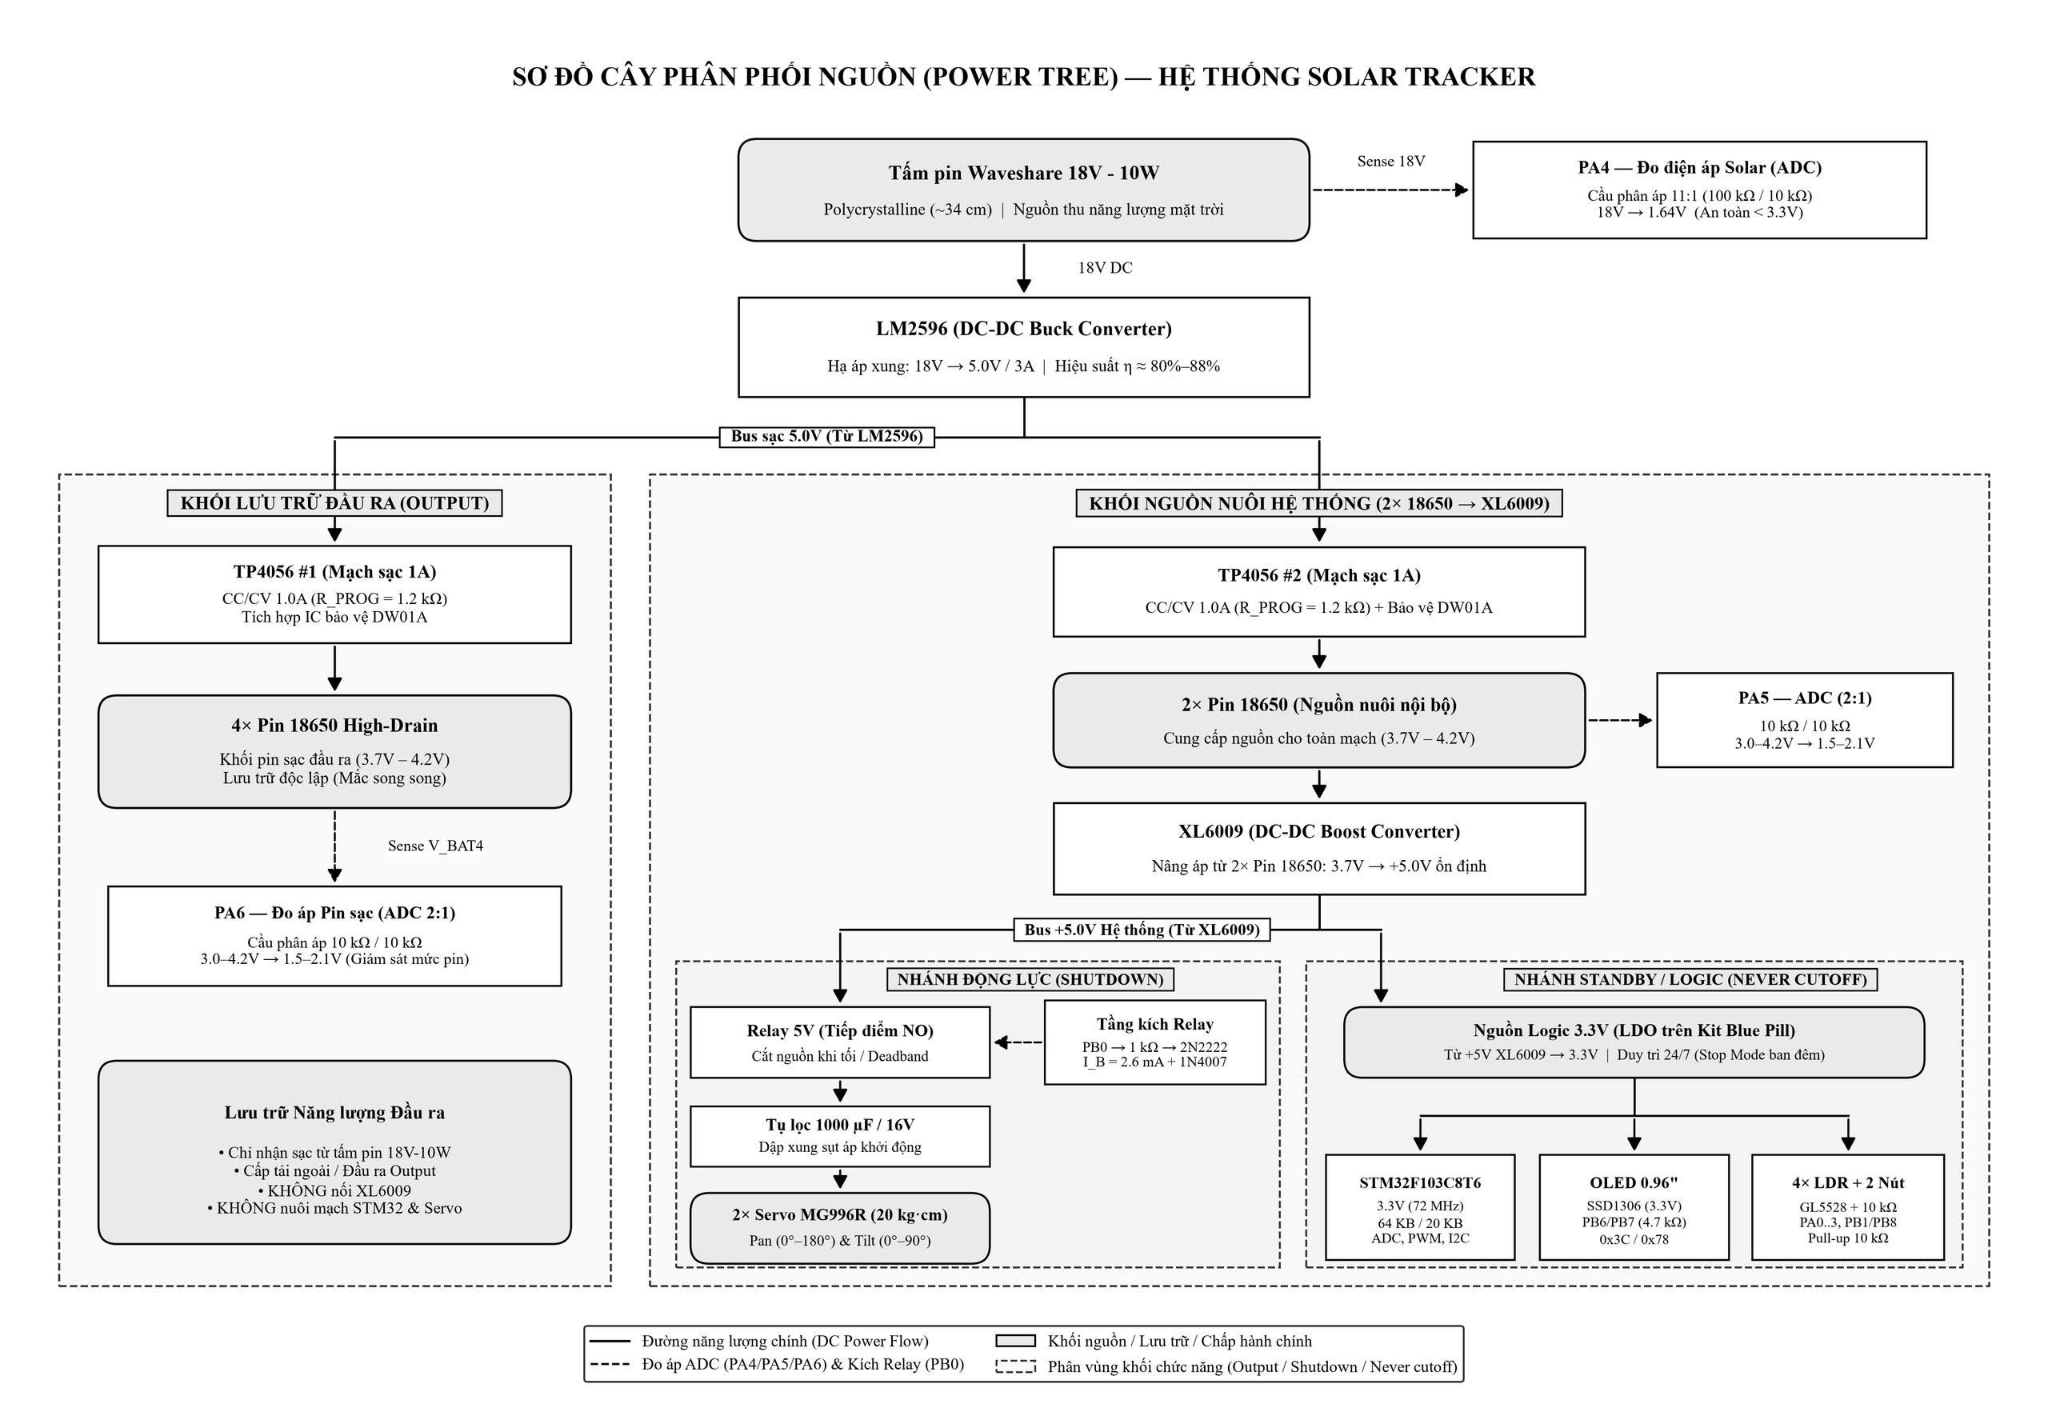
\includegraphics[width=0.92\textwidth,height=0.48\textheight,keepaspectratio]{images/img07_ch3_power_tree.png}
  \caption{Sơ đồ cây phân phối nguồn (Power Tree) hệ thống Solar Tracker.}
  \label{fig:img07}
\end{figure}

\textbf{Khối Lưu trữ Đầu ra (Output Storage --- 4x 18650):} Cụm 4x 18650 High-Drain nhận sạc từ LM2596 \ensuremath{\to} TP4056 \#1, đóng vai trò là \textbf{khối pin sạc lưu trữ đầu ra (Output) độc lập}, không nối qua XL6009 và không tham gia nuôi vi điều khiển hay cơ cấu Servo.

\textbf{Nhánh Standby / Logic (Never cutoff):} Từ nguồn nuôi \textbf{2x 18650}, điện áp được XL6009 nâng lên +5.0V và đi qua bộ LDO trên kit Blue Pill xuống 3.3V để duy trì liên tục cho STM32F103C8T6, OLED SSD1306, cụm LDR và nút nhấn (Stop Mode ban đêm khi thiếu nắng), bảo đảm không mất trạng thái điều khiển.

\textbf{Nhánh Động lực (Shutdown function):} Cũng lấy từ bus +5.0V đầu ra của XL6009, nguồn cấp cho hai động cơ MG996R 20kg đi qua tiếp điểm thường mở (NO) của Relay 5V. Khi tấm pin đã ổn định góc bám sáng trong vùng Deadband hoặc khi hệ thống về chế độ nghỉ ban đêm, chân PB0 nhả Relay để \textbf{cắt hoàn toàn nguồn cấp Servo}, cắt dòng tiêu thụ khi Servo không quay. Tụ hóa \textbf{1000\ensuremath{\mu}F / 16V} mắc ngay sau tiếp điểm Relay giúp bù năng lượng tức thời khi hai Servo khởi động, chống sụt áp đột ngột gây reset vi điều khiển.

\subsection{Thiết kế mạch sạc và khối pin Li-ion (2x TP4056, DW01A, 4x + 2x 18650)}

\textbf{Phân chia 2 cụm pin 18650 độc lập theo đúng chức năng:} Cụm \textbf{4x 18650 high-drain} (mắc song song 3.7V--4.2V) nhận sạc từ TP4056 \#1, chuyên tích trữ năng lượng mặt trời từ tấm pin 18V-10W làm khối lưu trữ đầu ra (\textit{Output Storage}) độc lập (không nối vào XL6009 và không nuôi mạch); cụm \textbf{2x 18650} sạc từ TP4056 \#2 và nối trực tiếp vào ngõ vào XL6009 để cấp nguồn nuôi +5.0V cho toàn bộ hệ thống (STM32, OLED, cảm biến và 2x Servo MG996R).

\textbf{Chu trình sạc an toàn 3 giai đoạn trên 2\texttimes{} TP4056:} Mỗi cụm pin được sạc độc lập bằng một module TP4056 (điện trở chọn dòng mặc định R\_PROG = 1.2 k\ensuremath{\Omega} cho dòng sạc tối đa 1 A) theo 3 bước tự động:

\textbf{1. Sạc mồi (Trickle Charge):} Khi pin xả sâu dưới 2.9V, mạch chỉ nạp dòng nhỏ (\ensuremath{\approx} 100 mA) để phục hồi cell an toàn trước khi sạc nhanh.

\textbf{2. Sạc dòng không đổi (CC):} Khi điện áp nằm trong dải 2.9V -- 4.2V, mạch giữ dòng nạp ổn định ở 1 A để sạc nhanh phần lớn dung lượng pin.

\textbf{3. Sạc áp không đổi (CV) \& tự ngắt:} Khi pin chạm mức đầy 4.2V, mạch giữ cố định mức áp này và giảm dần dòng nạp; khi dòng giảm về ngưỡng \ensuremath{\approx} 100 mA, quá trình sạc tự động dừng để tránh sạc quá mức.

\textbf{Mạch bảo vệ pin (DW01A + MOSFET kép):} Tích hợp sẵn trên module

TP4056, trong đó DW01A giám sát trạng thái pin và điều khiển MOSFET đóng/ngắt kịp thời khi xảy ra sạc quá áp (\ensuremath{\approx} 4.25V--4.30V), xả cạn dưới ngưỡng an toàn (\ensuremath{\approx} 2.4V--2.5V) hoặc quá dòng/ngắn mạch đầu ra.

\section{Giao tiếp Cơ bản I/O, Cảm biến, ADC \& Bus trên Bo mạch (Basic I/O, Sensors, ADC \& Board Bus)}

\subsection{Cảm biến quang trở LDR GL5528 và Giao tiếp ADC 12-bit}

\textbf{Cầu phân áp cảm biến sáng (PA0..PA3):} Bốn quang trở GL5528 đặt sau vách chữ thập, mỗi LDR mắc nối tiếp với điện trở cố định 10k\ensuremath{\Omega} xuống GND (đầu trên LDR nối 3.3V). Khi ánh sáng tăng, điện trở R\_LDR giảm mạnh, kéo điện áp về PA0..PA3 tăng theo biểu thức:

V\_ADC = 3.3V \texttimes{} [ 10k\ensuremath{\Omega} / (R\_LDR + 10k\ensuremath{\Omega}) ]

\textbf{Cầu phân áp đo điện áp bổ trợ trên Proteus (PA4..PA6):} Kênh PA4 sử dụng tỉ lệ 11:1 (100k\ensuremath{\Omega} / 10k\ensuremath{\Omega}) đo tấm pin 18V-10W (18V \ensuremath{\to} 1.64V, áp hở mạch 21.6V \ensuremath{\to} 1.96V, an toàn < 3.3V); kênh PA5 (10k\ensuremath{\Omega} / 10k\ensuremath{\Omega}, 2:1) đo khối 2x 18650 nguồn nuôi hệ thống; kênh PA6 (10k\ensuremath{\Omega} / 10k\ensuremath{\Omega}, 2:1) đo khối 4x 18650 pin sạc đầu ra (3.0V--4.2V \ensuremath{\to} 1.5V--2.1V).

\textbf{Độ phân giải ADC 12-bit (V\_REF = 3.3V):}

1 LSB = 3.3V / 2\textasciicircum{}12 = 3.3V / 4096 \ensuremath{\approx} 0.806 mV   

Sai số bước đọc: \textpm{}0.5 LSB \ensuremath{\approx} \textpm{}0.403 mV   

DR \ensuremath{\approx} 6.02 \texttimes{} 12 \ensuremath{\approx} 72.2 dB

\textbf{Thời gian lấy mẫu ADC:} Do cầu phân áp 100k\ensuremath{\Omega}/10k\ensuremath{\Omega} và quang trở khi trời râm có điện trở khá lớn, phần mềm cấu hình thời gian lấy mẫu dài (\textbf{71.5 chu kỳ xung ADC} --- ADC\_SAMPLETIME\_71CYCLES\_5, ADCCLK \ensuremath{\le} 14 MHz) để điện áp đọc về ổn định. Thực tế mạch nên gắn thêm tụ lọc 10 nF tại chân ADC để giảm nhiễu từ Servo.

\subsection{Tầng kích Relay (Drive Relays) --- Transistor 2N2222 \& Dập xung 1N4007}

Do dòng hút cuộn Relay 5V (\ensuremath{\approx} 70--80 mA) vượt quá khả năng chịu tải chân GPIO STM32 (\ensuremath{\le} 25 mA), mạch sử dụng tầng đệm transistor NPN \textbf{2N2222} (Q1):
\begin{itemize}[leftmargin=1.5em,itemsep=3pt]
  \item \textbf{Tính toán dòng Base kích bão hòa:} Tín hiệu 3.3V từ PB0 qua điện trở hạn dòng R5 = 1k\ensuremath{\Omega} cấp dòng Base:
\end{itemize}

I\_B = (V\_GPIO - V\_BE(sat)) / R5 = (3.3V - 0.7V) / 1000\ensuremath{\Omega} = 2.6 mA

Với dòng tải cuộn hút I\_C \ensuremath{\approx} 75 mA và hệ số khuếch đại tối thiểu \ensuremath{\beta}\_min \ensuremath{\ge} 75, mức dòng cần để chớm dẫn là \ensuremath{\approx} 1.0 mA. Việc thiết kế I\_B = 2.6 mA đảm bảo 2N2222 dẫn \textbf{bão hòa hoàn toàn} (V\_CE(sat) < 0.3V), giảm phát nhiệt và đóng Relay dứt khoát.
\begin{itemize}[leftmargin=1.5em,itemsep=3pt]
  \item \textbf{Diode dập xung ngược 1N4007 (D1):} Mắc song song ngược chiều với cuộn dây RL1 để xả xung điện áp ngược sinh ra khi ngắt cuộn dây, bảo vệ transistor 2N2222 không bị đánh thủng.
  \item \textbf{Tụ lọc ổn áp 1000\ensuremath{\mu}F / 16V (C1):} Đặt tại đầu ra tiếp điểm NO cấp nguồn 5V cho 2x Servo MG996R để dập xung sụt áp khởi động.
\end{itemize}

\subsection{Bus giao tiếp trên bo mạch (Board Bus) --- I2C1 điều khiển OLED 0.96"}

\textbf{Chuẩn giao tiếp:} Bus I2C1 trên hai chân \textbf{PB6 (SCL)} và \textbf{PB7 (SDA)}, chế độ Fast Mode 400 kHz, cấu hình Open-Drain với hai điện trở kéo lên \textbf{4.7k\ensuremath{\Omega}} (R6, R7) lên nguồn 3.3V (I\_sink \ensuremath{\approx} 3.3V / 4.7k\ensuremath{\Omega} \ensuremath{\approx} 0.7 mA).

\textbf{Hiển thị ngoại vi:} Màn hình OLED 0.96" SSD1306 (128\texttimes{}64 pixels), địa chỉ 7-bit \textbf{0x3C} (địa chỉ ghi 8-bit \textbf{0x78}), cập nhật góc Pan/Tilt, giá trị LDR, \% pin và điện áp Solar.

\subsection{Nút nhấn giao tiếp và chống dội phím (Bổ trợ trên Proteus)}

Hai nút nhấn MODE (PB1) và PARK 90\textdegree{} (PB8) đấu kiểu Active-Low với điện trở kéo lên ngoài \textbf{10k\ensuremath{\Omega}} (R8, R9) lên 3.3V. Phần mềm áp dụng bộ định thời \textbf{chống dội phím tối thiểu 20 ms} (có thể lắp thêm tụ 0.1\ensuremath{\mu}F song song nút nhấn nếu môi trường ngoài trời có nhiễu cao).

\section{Thiết kế Sơ đồ nguyên lý, Kết nối, Kiểm tra và Danh mục Linh kiện (Schematic Design, Connectors, Checklist \& BOM)}

\subsection{Phân khối Sơ đồ nguyên lý \& Quy ước đặt tên (Name Identifier)}

\textbf{Phân tách 9 khung khối chức năng trên Proteus:} LDR, SOLAR, STM32, OLED, BUTTON, RELAY, SERVO, NGUON NUOI (2x 18650 nối XL6009 nuôi hệ thống) và PIN SAC (4x 18650 tích trữ đầu ra Output). Kết nối giữa các khối thực hiện qua nhãn lưới (\textit{Net Labels}) giúp mạch sáng rõ, dễ rà soát lỗi.

\textbf{Quy ước định danh (Reference Designator):} R (Điện trở: R1..R4 10k\ensuremath{\Omega} LDR, R5 1k\ensuremath{\Omega} Relay, R6..R7 4.7k\ensuremath{\Omega} I2C, R8..R9 10k\ensuremath{\Omega} nút nhấn); C (Tụ điện C1 1000\ensuremath{\mu}F); D (Diode 1N4007); Q (Transistor 2N2222); RL (Relay 5V); U (MCU \& Module nguồn LM2596, TP4056, XL6009); B/BT (Tấm pin / Cell 18650).

Sơ đồ nguyên lý phân khối trên phần mềm Proteus được trình bày tại các hình dưới đây:

\begin{figure}[H]
  \centering
  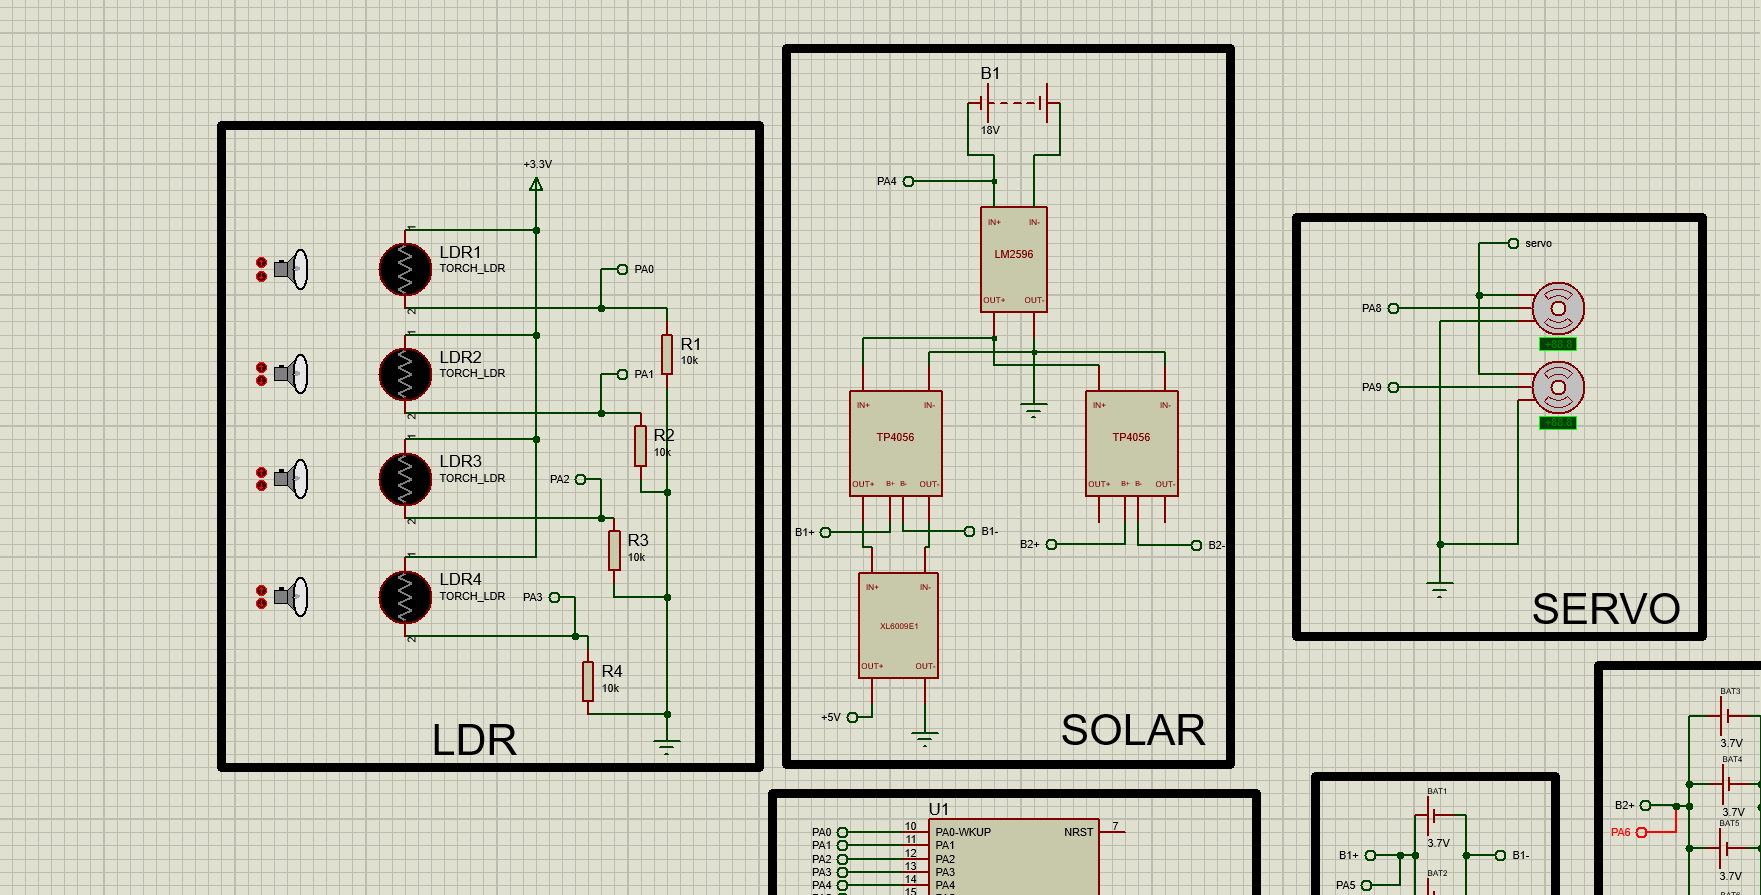
\includegraphics[width=0.92\textwidth,height=0.48\textheight,keepaspectratio]{images/img08_ch3_proteus_phan1_ldr_solar_servo.png}
  \caption{Sơ đồ nguyên lý Proteus --- Cụm cảm biến LDR, khối nguồn Solar và cơ cấu Servo.}
  \label{fig:img08}
\end{figure}

\begin{figure}[H]
  \centering
  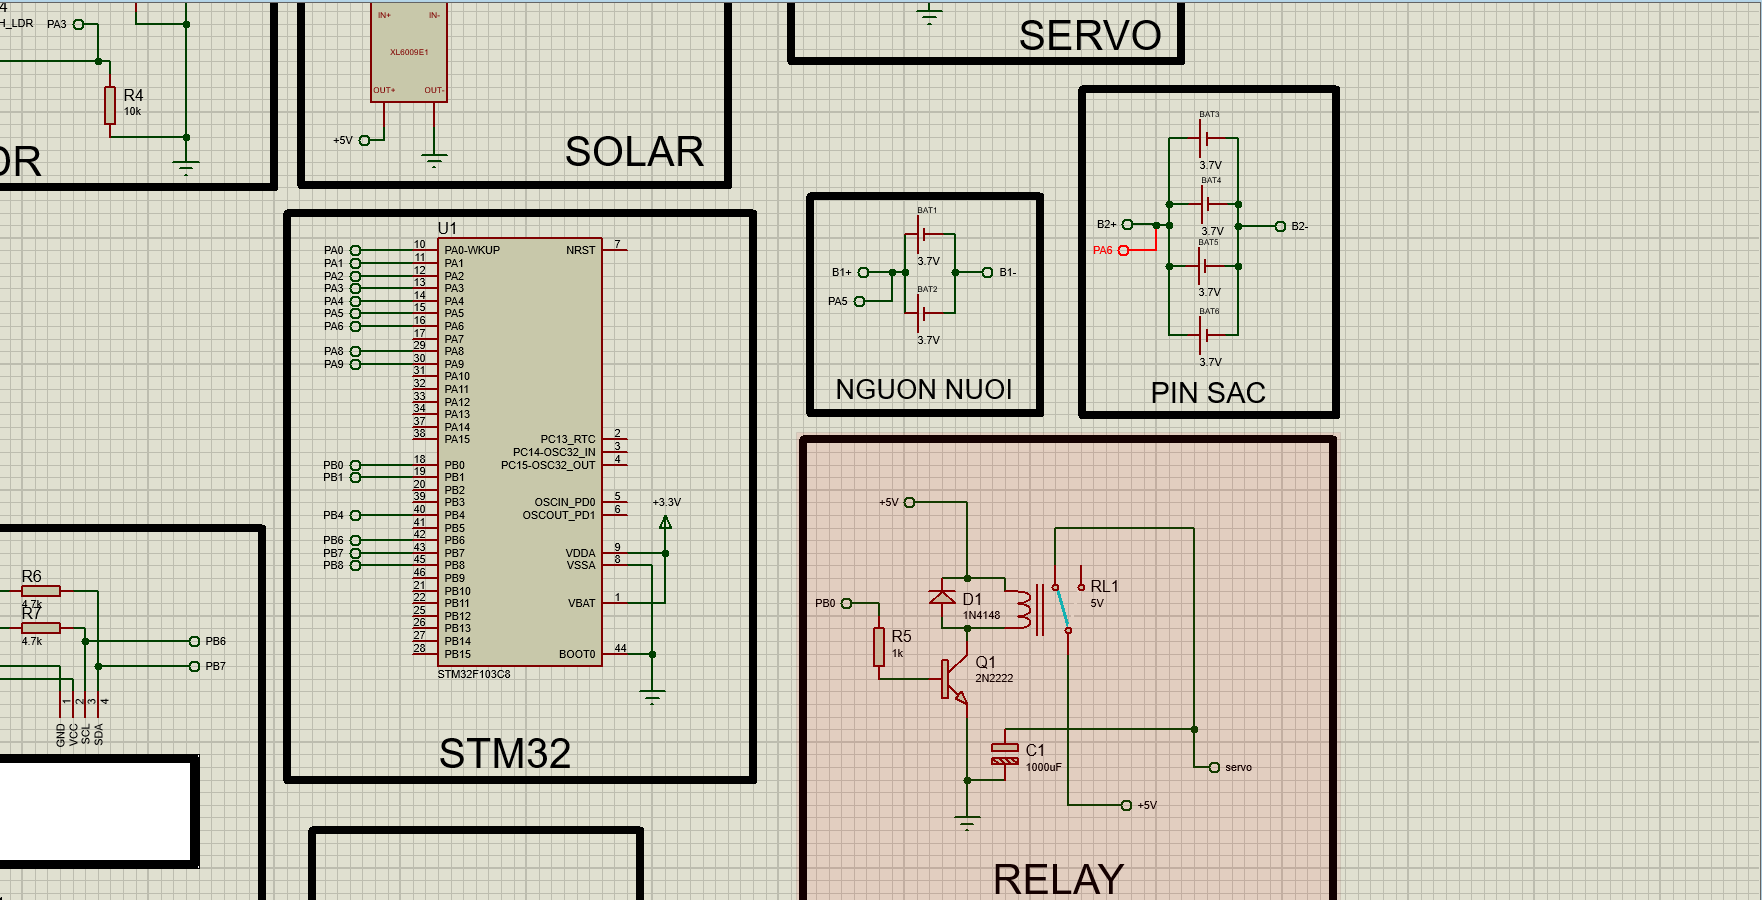
\includegraphics[width=0.92\textwidth,height=0.48\textheight,keepaspectratio]{images/img09_ch3_proteus_phan2_stm32_pin_relay.png}
  \caption{Sơ đồ nguyên lý Proteus --- Cụm vi điều khiển STM32, nguồn nuôi, pin sạc và Relay.}
  \label{fig:img09}
\end{figure}

\begin{figure}[H]
  \centering
  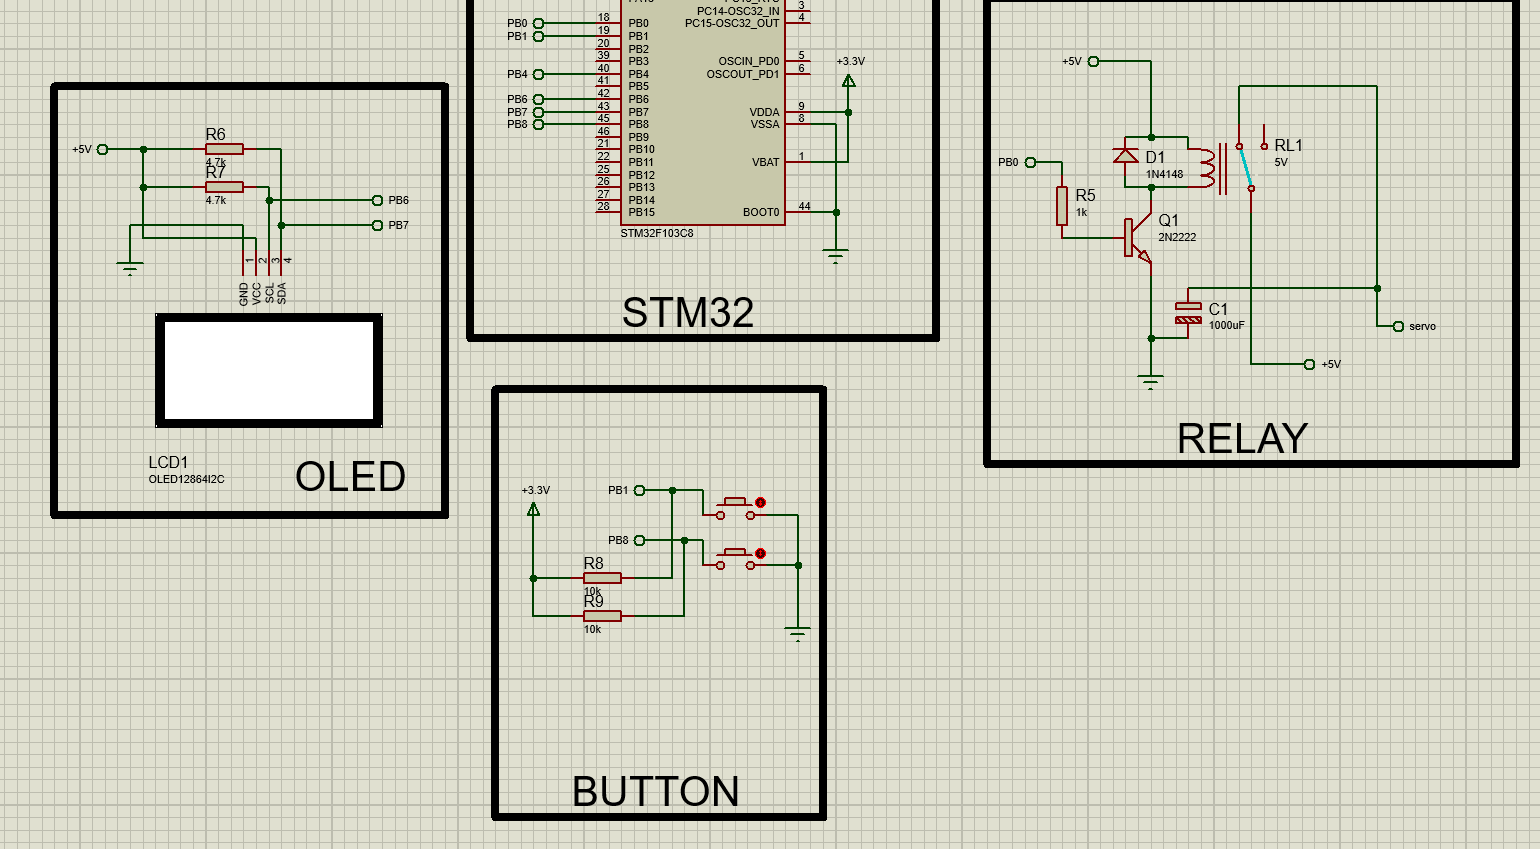
\includegraphics[width=0.92\textwidth,height=0.48\textheight,keepaspectratio]{images/img10_ch3_proteus_phan3_oled_button_relay.png}
  \caption{Sơ đồ nguyên lý Proteus --- Cụm hiển thị OLED I2C, nút nhấn và tầng kích Relay.}
  \label{fig:img10}
\end{figure}

\subsection{Đầu nối (Connectors), Đấu dây (Cable/Wiring) \& Yêu cầu Lắp đặt ngoài trời}

\textbf{Đầu nối phân loại theo dòng và tín hiệu:} Dùng Domino / Terminal Block 2-pin KF301 (5.08mm) cho ngõ vào tấm pin 18V-10W và dây công suất pin 18650 (chịu dòng \ensuremath{\ge} 5A); Header 2.54mm (3-pin đực) cho 2 Servo MG996R; Header 2.54mm (4-pin cái) cho OLED I2C; Header 4-pin riêng cho cổng nạp SWD; và đế pin 18650 dây ra 20 AWG.

\textbf{Phân màu \& Đấu dây (Wire Numbering / Color Coding):} Dây \textbf{Đỏ} cho đường nguồn dương (+18V, +5V, +3.3V); dây \textbf{Đen} nối đất theo nguyên tắc \textbf{Star Ground} (gom dây GND dòng cao của Servo về thẳng cực âm tụ 1000\ensuremath{\mu}F/nguồn chính, tách riêng với GND tín hiệu LDR/OLED); dây \textbf{Vàng/Cam} cho PWM và I2C SDA; dây \textbf{Xanh} cho ADC LDR và I2C SCL.

\textbf{Yêu cầu cơ khí \& lắp đặt ngoài trời (theo Requirement Forms PDF):} Kích thước tổng thể mô hình khoảng \textbf{250 \texttimes{} 250 \texttimes{} 400 mm}, khối lượng \textbf{2.0 -- 2.5 kg}. Bó dây từ tấm pin 34cm và cụm 4 LDR đi qua khớp quay phải chừa độ chùng (\textit{service loop}) tránh căng đứt khi quét Pan 0\textdegree{}--180\textdegree{} và Tilt 0\textdegree{}--90\textdegree{}. Vị trí lắp đặt cần thoáng đãng, quay \textbf{hướng Nam}, \textbf{không bị bóng râm che khuất từ 7h00--16h00} (tránh hiện tượng \textit{hunting} đảo góc) và \textbf{tránh khe gió hút giữa các tòa nhà cao tầng} để bảo vệ cơ cấu trục mang tấm pin 34 cm.

\subsection{Bảng kiểm tra Sơ đồ nguyên lý (Schematic Checklist)}

{
\small
\setlength{\LTleft}{0pt}\setlength{\LTright}{0pt}
\begin{longtable}{>{\raggedright\arraybackslash}p{0.060\textwidth}>{\raggedright\arraybackslash}p{0.220\textwidth}>{\raggedright\arraybackslash}p{0.260\textwidth}>{\raggedright\arraybackslash}p{0.380\textwidth}}
\toprule
\textbf{STT} & \textbf{Hạng mục kiểm tra (}\textbf{\textit{Checklist}}\textbf{)} & \textbf{Tiêu chuẩn đạt chuẩn kỹ thuật} & \textbf{Trạng thái / Ghi chú} \\
\midrule
\endfirsthead
\toprule
\textbf{STT} & \textbf{Hạng mục kiểm tra (}\textbf{\textit{Checklist}}\textbf{)} & \textbf{Tiêu chuẩn đạt chuẩn kỹ thuật} & \textbf{Trạng thái / Ghi chú} \\
\midrule
\endhead
\bottomrule
\endfoot
\bottomrule
\endlastfoot
1 & \textbf{Nguồn cấp \& Đất (VCC/GND)} & Phân rõ miền 18V, 5V\_CHG, 5V\_SERVO, 3.3V; đấu \textit{Star Ground} nhánh động lực. & Đạt (có tụ 1000\ensuremath{\mu}F sau Relay) \\
2 & \textbf{Cực tính linh kiện có cực} & Kiểm tra 1N4007, tụ hóa 1000\ensuremath{\mu}F, chân E-B-C 2N2222 và cực +/- cell 18650. & Cần sửa X-Mirror pin trên Proteus \\
3 & \textbf{Giới hạn áp ngõ vào MCU} & Mọi chân PA0..PA6, PB1, PB8 không vượt quá 3.3V (bảo vệ chân ADC). & Cần bổ sung phân áp PA4, PA5, PA6 \\
4 & \textbf{Điện trở kéo lên (Pull-up)} & Bus I2C1 có R6=R7=4.7k\ensuremath{\Omega}; 2 nút nhấn PB1, PB8 có R8=R9=10k\ensuremath{\Omega} lên 3.3V. & Đạt \\
5 & \textbf{Công suất \& định mức linh kiện} & LM2596 (\ensuremath{\le}3A), TP4056 (1A, bảo vệ DW01A), tụ 16V, 2N2222 dẫn bão hòa. & Đạt \\
6 & \textbf{Cấu hình khởi động MCU} & Chân BOOT0 kéo xuống GND (chạy Flash); chân NRST có tụ lọc 100nF. & Đạt \\
7 & \textbf{Cách ly dòng lớn \& Servo} & Đường dây 2x MG996R qua tiếp điểm NO Relay, tách xa dây analog LDR. & Đạt \\
8 & \textbf{Nhãn lưới \& Định danh đầy đủ} & Đầy đủ Name Identifier (R, C, D, Q, U, RL, B), giá trị và khung phân khối. & Đạt \\
\end{longtable}
}

\subsection{Danh mục Linh kiện (Bill of Materials --- BOM)}

Bảng BOM dưới đây tổng hợp toàn bộ linh kiện phần cứng, nguồn lưu trữ và kết cấu cơ khí cho hệ thống hoàn chỉnh với tổng kinh phí \textbf{1.280.000 VNĐ}, nằm trọn trong ngân sách dự toán \textbf{1.000.000 -- 1.500.000 VNĐ} của nhóm:

{
\footnotesize
\setlength{\LTleft}{0pt}\setlength{\LTright}{0pt}
\begin{longtable}{>{\raggedright\arraybackslash}p{0.050\textwidth}>{\raggedright\arraybackslash}p{0.110\textwidth}>{\raggedright\arraybackslash}p{0.160\textwidth}>{\raggedright\arraybackslash}p{0.290\textwidth}>{\raggedright\arraybackslash}p{0.070\textwidth}>{\raggedright\arraybackslash}p{0.110\textwidth}>{\raggedright\arraybackslash}p{0.130\textwidth}}
\toprule
\textbf{STT} & \textbf{Ref Des} & \textbf{Hạng mục} & \textbf{Mô tả / Thông số} & \textbf{SL} & \textbf{Đơn giá (VNĐ)} & \textbf{Thành tiền (VNĐ)} \\
\midrule
\endfirsthead
\toprule
\textbf{STT} & \textbf{Ref Des} & \textbf{Hạng mục} & \textbf{Mô tả / Thông số} & \textbf{SL} & \textbf{Đơn giá (VNĐ)} & \textbf{Thành tiền (VNĐ)} \\
\midrule
\endhead
\bottomrule
\endfoot
\bottomrule
\endlastfoot
1 & U1 & Vi điều khiển trung tâm & STM32F103C8T6 Blue Pill (Cortex-M3 72MHz, 64KB Flash, 20KB SRAM) & 1 & 65.000 & 65.000 \\
2 & STLINK & Mạch nạp \& gỡ lỗi & Mạch nạp ST-Link V2 Mini (giao tiếp SWD) & 1 & 55.000 & 55.000 \\
3 & B1 & Tấm pin năng lượng mặt trời & Waveshare Polycrystalline 18V - 10W (cạnh \textasciitilde{}34 cm) & 1 & 240.000 & 240.000 \\
4 & M1, M2 & Động cơ Servo bám sáng & Servo MG996R công suất lớn 20 kg\ensuremath{\cdot}cm (Pan 0\textdegree{}--180\textdegree{}, Tilt 0\textdegree{}--90\textdegree{}) & 2 & 95.000 & 190.000 \\
5 & OLED1 & Màn hình hiển thị & OLED 0.96" I2C (SSD1306, 128\texttimes{}64, địa chỉ 0x3C / 0x78) & 1 & 65.000 & 65.000 \\
6 & U2 & Mạch hạ áp DC-DC & Module Buck LM2596 (18V \ensuremath{\to} 5V, tối đa 3A) & 1 & 25.000 & 25.000 \\
7 & U3, U4 & Mạch sạc pin Li-ion & Module sạc TP4056 1A tích hợp IC bảo vệ DW01A & 2 & 15.000 & 30.000 \\
8 & U5 & Mạch tăng áp DC-DC & Module Boost XL6009 (nâng áp khối 2x 18650 3.7V \ensuremath{\to} 5V nuôi mạch \& Servo) & 1 & 30.000 & 30.000 \\
9 & BT1..BT4 & Pin sạc lưu trữ đầu ra & Cell Li-ion 18650 High-Drain (3.7V--4.2V, 2500mAh --- Output độc lập) & 4 & 55.000 & 220.000 \\
10 & BT5, BT6 & Pin nguồn nuôi hệ thống & Cell Li-ion 18650 (cấp vào XL6009 nuôi STM32, OLED \& 2x Servo) & 2 & 45.000 & 90.000 \\
11 & BH1, BH2 & Đế pin 18650 & Đế 4 cell + Đế 2 cell 18650 (dây ra 20 AWG) & 2 & 20.000 & 40.000 \\
12 & RL1,Q1,D1,C1 & Khối kích Relay \& lọc nguồn & Relay 5V + BJT 2N2222 + Diode 1N4007 + Tụ 1000\ensuremath{\mu}F/16V & 1 bộ & 25.000 & 25.000 \\
13 & LDR, R, SW & Cảm biến \& thụ động & 4\texttimes{} LDR GL5528, trở 10k/100k/4.7k/1k\ensuremath{\Omega}, tụ 10nF, 2 nút nhấn & 1 bộ & 35.000 & 35.000 \\
14 & J, WIRE & Đầu nối, bo \& dây dẫn & PCB/Testboard đồng, Header 2.54mm, Domino KF301, dây động lực & 1 bộ & 50.000 & 50.000 \\
15 & MECH & Khung cơ khí \& gá Pan-Tilt & Giá đỡ Pan-Tilt hợp kim + đế 250\texttimes{}250\texttimes{}400 mm \& vách chữ thập & 1 bộ & 120.000 & 120.000 \\
\midrule
\textbf{Tổng} & \textbf{---} & \textbf{Tổng chi phí dự toán (BOM)} & \textbf{Đạt định mức ngân sách 1.000.000 -- 1.500.000 VNĐ} & \textbf{---} & \textbf{---} & \textbf{1.280.000} \\
\end{longtable}
}

\end{document}
